% arara: xelatex
% arara: xelatex
% arara: xelatex


% options:
% thesis=B bachelor's thesis
% thesis=M master's thesis
% czech thesis in Czech languagef
% english thesis in English language
% hidelinks remove colour boxes around hyperlinks

\documentclass[thesis=B,english]{FITthesis}[2019/12/23]

%\usepackage[utf8]{inputenc} % LaTeX source encoded as UTF-8
% \usepackage[latin2]{inputenc} % LaTeX source encoded as ISO-8859-2
% \usepackage[cp1250]{inputenc} % LaTeX source encoded as Windows-1250

% \usepackage{subfig} %subfigures
% \usepackage{amsmath} %advanced maths
% \usepackage{amssymb} %additional math symbols

\usepackage{dirtree} %directory tree visualisation
\usepackage{graphicx}
\usepackage{tocbibind}
\usepackage[T1]{fontenc}
\usepackage{float}
\usepackage{pdfpages}

\graphicspath{ {./images/} }

% % list of acronyms
% \usepackage[acronym,nonumberlist,toc,numberedsection=autolabel]{glossaries}
% \iflanguage{czech}{\renewcommand*{\acronymname}{Seznam pou{\v z}it{\' y}ch zkratek}}{}
% \makeglossaries

% % % % % % % % % % % % % % % % % % % % % % % % % % % % % % 
% EDIT THIS
% % % % % % % % % % % % % % % % % % % % % % % % % % % % % % 

\department{Department of Software Engineering}
\title{Cluster infrastructure for LearnShell}
\authorGN{Samuel} %author's given name/names
\authorFN{Majoroš} %author's surname
\author{Samuel Majoroš} %author's name without academic degrees
\authorWithDegrees{Samuel Majoroš} %author's name with academic degrees
\supervisor{Ing. Jakub Žitný}
\abstractEN{The main goal of this thesis is to present a functional cluster infrastructure for the LearnShell 2.0 project used by the Czech Technical University in Prague. To achieve this, we have described the current infrastructure and scrutinized today's pre-eminent technologies for container orchestration. As a result, we present a basic cluster on which the LearnShell project is to be hosted, and have also defined CI/CD routines for the services contained therein by utilizing Gitlab CI. We have documented our code thoroughly and display our code in a separate repository.}
\abstractCS{Hlavným cieľom tejto práce je uvedenie funkčnej klastrovej infraštruktúry pre projekt LearnShell 2.0, ktorý je používaný Českou Technickou Univerzitou v Prahe. Aby sme dosiahli tento cieľ, najprv sme opísali súčasnú infraštruktúru a posúdili dnešné najznámejšie technológie pre kontajnerovú orchestráciu. Výsledkom je jednoduchý klaster, na ktorom bude LearnShell hostovaný, a zadefinovaný je CI/CD proces pre v klastri existujúce servisy. Náš kód pozorne zdokumentovali a kód uvádzame vo svojom vlastnom repozitári.}
\placeForDeclarationOfAuthenticity{Prague}
\keywordsCS{Kubernetes, Helm, Docker, Docker Swarm, Gitlab CI, Google Cloud, Linux, LearnShell}
\keywordsEN{Kubernetes, Helm, Docker, Docker Swarm, Gitlab CI, Google Cloud, Linux, LearnShell}
\declarationOfAuthenticityOption{1} %select as appropriate, according to the desired license (integer 1-6)
% \website{https://gitlab.fit.cvut.cz/learnshell-2.0/ls-cluster/tree/majorsam} %optional thesis URL



\begin{document}



% \newacronym{CVUT}{{\v C}VUT}{{\v C}esk{\' e} vysok{\' e} u{\v c}en{\' i} technick{\' e} v Praze}
% \newacronym{FIT}{FIT}{Fakulta informa{\v c}n{\' i}ch technologi{\' i}}

\setsecnumdepth{part}
\chapter{Introduction}

As we become ever reliant on internet-based technology in our daily lives, it stands to reason that there is a pervasive demand for software that is safe, accessible, and most importantly, dependable. More and more, we are growing accustomed to using the internet for even the most trivial of things, such as ordering food or looking up the correct spelling of certain words. Therefore, web applications are ever-increasingly throttled by an uncountable amount of requests from users, and it is of great importance that technology adapts to this challenge by employing new methods of creating an infrastructure that is scalable in a way that makes it impossible to be overwhelmed by too many requests to the point of system failure. In this thesis, we shall attempt to explain the theory behind, as well as the need for, containerization and orchestration as catch-all solutions to many problems troubling today's web applications. More specifically, we shall try and implement a basic cluster on which the LearnShell portal of the Czech Technical University in Prague could run in the near future. 

In summary, these will be the main goals of the thesis:
\begin{itemize}
  \setlength\itemsep{0em}
  \item Analyze the current infrastructure architecture of LearnShell.
  \item Explain the virtues of containerization and orchestration, as well as their history.
  \item Compare existing orchestration technologies used in practice as well as their suitability for orchestrating LearnShell containers.
  \item Implement a basic cluster based on cutting-edge orchestration systems.
  \item Explore implementation of continuous integration and continuous deployment in LearnShell, specifically the newly created cluster.
\end{itemize}

\section{Motivation}

This thesis is motivated by current inefficiencies in the LearnShell system related to scalability, availability, and load balancing, as well as the current absence of complex logging, monitoring, and reporting. By researching current state-of-the-art technologies for containerization and orchestration, our aim is to present a solution to many of these problems by migrating to a cluster-based architecture. Such a solution would not only enable us to benefit from high availability and ease of scaling LearnShell components depending on our day-to-day needs but also potentially give us a platform for effective CI/CD processes. During the course of implementing our cluster, we shall try and explore all of these avenues and find ways to benefit from them.


\setsecnumdepth{all}
\chapter{Architecture of LearnShell}

In this chapter, we shall take a closer look at the architecture of LearnShell.

Before that, let us briefly describe its history. The first version of LearnShell was designed and built by Karel Jilek, a student of the Czech Technical University in Prague. In his bachelor's thesis, titled "Command and script testing system for bash language", he explains that the goal of this system would be to create an environment that would be able to verify the validity of a bash script by simply comparing the output of that script with the output provided by the system. \cite{learnshell-jilek} Later on, LearnShell would be used in the course "Programming in Shell 1" to evaluate assignments and exams specific to Bash programming. Eventually, a newer version, called "LearnShell 2.0" was introduced. This version would build upon the old one, providing new features, such as a plagiarism detection system, a logging system, as well as introducing a newer front-end design. And last but not least, a cluster would be created on which the application was to be deployed. In this chapter (and by extension this thesis), we shall focus on describing the state of affairs in the 2.0 version, as this is the version on which work is being done at the moment.

Now, let us begin with an overview of the architecture. Next, we shall focus on each separate piece of the puzzle as well as the tech stack in use.

\clearpage

\section{Overview}

The current production-ready version of LearnShell is composed of six containers that are connected to each other on their local network, alongside an evaluator service that runs on its own server. Each of those services fulfills a specific role, as we will elaborate in the following subsections. In practice, the term for this is "microservice architecture", which can be succinctly described as a collection of small, autonomous services that work together. \cite{building-microservices} 
\newline
In general, such an architecture adheres to principles of deployability and modifiability. \cite{building-microservices,architecting-chen} Meaning that by compartmentalizing your application into several smaller pieces, one can easily modify and later, deploy one part of the entire application without having to include the other parts, therefore avoiding issues such as having to compile the entire application after changing just one small piece of it. It is therefore only logical that in the case of LearnShell, lightweight, easily configurable containers, in the form of Docker containers, are used to divide the application into smaller parts, or packages. Not only that, but these containers are fairly simple to get running via configuration files. These containers communicate with each other via HTTP requests that work like glue holding the entire application together. \cite{microservices}

In the case of LearnShell, six containers in total are used as of right now. In the following sections, we shall briefly explain the functionality of each containerized package (plus the evaluator) in concise terms, as well as the technologies used by those packages. However, to get a full understanding of the inner workings of the application, it is advised to read the bachelor's thesis of Karel Jilek on this subject.

As a side note, even though the current architecture of LearnShell leans towards a microservices-based one, it is definitely not an example of an application purely made of microservices; for example, the backend service combines several features, such as an administration panel and a GraphQL together, and as such doesn't fit the bill of a microservice and is closer to a monolithic application in its scope. Nonetheless, the generator and evaluator only fulfill one specific role each and are therefore much closer to the definition of a microservice. Since LearnShell is production-ready software, it is quite natural that it doesn't perfectly adhere to one paradigm, as that is nigh-on-impossible to achieve in practice.

\section{Architecture}

In this section, we shall explore the LearnShell architecture, its components, and technologies used, all of which except for the evaluator are currently containerized and as such are prime candidates for migration into a cluster-based architecture, which we shall cover later.

\subsection{Proxy server}

For the purpose of receiving incoming traffic and redirecting it, a container is used as a proxy server, which redirects requests received from the client, and points them toward containers for further processing, and sending back responses to the client received from these same containers as if it was by itself their origin, therefore fulfilling the role of a reverse proxy. \cite{proxies} A subdomain of the fit.cvut.cz domain is assigned to the ip address of this proxy server.

For all this, nginx was chosen as the most suitable candidate. As of 2021, Nginx is the most commonly used web server and is renowned for its performance and ease of use. \cite{netcraft} Naturally, a well-maintained Docker image is available publicly on DockerHub, and there is no reason not to use it in production in this application, as well.

\subsection{Front end}

This container contains the code for the front end side of the application. As well as responding with the HTTP response, including assets such as CSS files and images to display on the client side, it also sends GraphQL queries to other containers, for example, to create or display assignments. 

It is built entirely with Next.js, a modern JavaScript framework based on React, improving on it by adding most importantly a built-in routing system (by default, React does not contain one, and additional libraries, such as React Router, must be used) and several additional features such as server-side rendering or faster page loading by virtue of automatic code splitting.

\subsection{Back end}

The code in this container represents the data access layer of the application. Among its functionalities is writing and reading data to the database (such as users and assignments) and communicating with the generator and evaluator services for the purpose of creating randomized data for validation of Bash scripts and evaluating the outputs of these scripts by comparing them with the generated data. \cite{learnshell-borsky} The back end also communicates with KOS, our student information system, and integration with the system for grades and evaluations, Grades, is planned for the future.

The entire back end is built in Django, a web framework written in Python adhering to the model-view-presenter architectural pattern. In addition, the container contains several Bash scripts to ensure, between other things, connection and migration of data to the database, as well as configuration files for the web server.

\subsection{Distributed task queue}

In order to enable LearnShell to parallelize tasks related to the generation of inputs and evaluation of Bash scripts, a distributed task queue is used. This comes in handy because not all of those tasks are completed in the same time horizon; therefore by using the distributed tasks queue, long-running tasks are "worked on" by the services to which these tasks are assigned, namely generator or evaluator, while simple tasks such as data retrieval are still executed without having to wait for long-running tasks to finish.

The technologies used here are the Python library Celery, which provides all the tools required for running a queue on LearnShell, while we use a key-value database, Redis as an in-memory database on which the information regarding jobs is stored in that queue until these jobs are finished. Both the generator and the evaluator use their own distributed task queue, with the generator using a containerized one and the evaluator running it on its own server for now.

\subsection{Database}

Alongside Redis, the only stateful service in the application, a SQL database is used to store all important data persistently. The database contains information regarding users and their privileges, all the jobs performed by Celery, assignments, and exams created by teachers, as well as submissions by students. LearnShell utilizes the PostgreSQL engine, although there is no particular reason to use it in particular as opposed to other SQL engines; it boiled down to the initial author's preference.

\subsection{Generator}

To elaborate on what was already mentioned in the back end subsection, the function of the generator service is the generation of randomized data for validation of LearnShell assignments and exams. 

Solely for this reason, the LearnShell Input-Describing Language (LI-DL for short) was developed, a sort of minimalistic domain-specific language with a syntax similar to JSON that generates custom assignments as well as test cases, which the evaluator compares with the output of a shell script that is turned in by the user. \cite{learnshell-jilek}  
 
\subsection{Evaluator}

The evaluator, as befits its name, fulfills the role of a service that assesses each submission made by the user. It does so by creating a chroot jail, which is essentially a simulated root environment running on a directory; this way, the directory in question is isolated from the rest of the computer, protecting the computer from potential destructive effects of certain commands, such as the famous fork bomb. \cite{unix-handbook} It checks for criteria such as whether the user-created or deleted the correct files, whether the files created have the correct permissions, or the outputs (and the streams through which they are passed) of the scripts submitted.

Currently, the evaluator runs on its own server and therefore is the only service which is not packaged inside of a container. Note that this is why the evaluator will \textbf{not} be a part of our cluster (both Docker Swarm and Kubernetes require applications to be running in containers); instead, the cluster should for now, connect to the server on which the evaluator is running. Once the evaluator is containerized, there is no reason not to include it within our cluster.

\section{Potential improvements}

Lastly, let us pick up on what was started in the introduction of our thesis, and expand on current inefficiencies and potential improvements to the LearnShell portal. Incidentally, all of these inefficiencies can be handled either completely or in part by utilizing a cluster-based architecture for our application. Be advised that we use several terms here which are not yet formally defined in our thesis, such as Docker or CI/CD; to see their definitions and use cases, consult the following chapters. This section merely serves as an introduction to the problems we are attempting to solve, as well as potential additions to LearnShell as it is right now.

\subsection{High availability}

An extremely important aspect of modern software is availability, which denotes the period of time when a service is available and is often expressed as a percentage indicating how much time the application spends in a working state. \cite{what-is-high-availability} By extension, a highly available application is simply an application that spends as much time as possible up and running, with the downtime being so negligible that it will not be noticed by users at all.

Orchestration technologies were built exactly with high availability in mind; by running several replicas of components of LearnShell, all our components are made redundant, meaning that if one component of LearnShell fails, its replica rises immediately to fulfill the same role. Thus, we eliminate any single points of failure, and the system can be kept up and running even under extreme loads.

\subsection{Load balancing}

To follow up on the previous subsection, load balancing should be mentioned as another powerful feature of architectures that run several replicas of their components. Generally, load balancing is defined as the methodical and efficient distribution of network traffic across multiple servers in a server farm; in our case, we may replace the word "server" with "workload" and "server farm" with "cluster". \cite{citrix} By creating and configuring the network of our cluster, we can make our cluster manage the incoming traffic, that is web requests of all kinds, in a resourceful way. For example, in case of an unusually high amount of requests, load balancing algorithms would redirect these requests to those workloads within the cluster that are least burdened at the moment, balancing the number of requests and ensuring that there are minimal bottlenecks.

It should be noted that by itself, the nginx server used by LearnShell has load balancing capabilities. However our architecture falls short by not utilizing multiple replicas for critical parts of the application, and as such there can be no real distribution of the requests being received by LearnShell at the moment.

\subsection{CI/CD}

An implementation of a CI/CD pipeline has no real disadvantages and many potential advantages and future opportunities. We will be discussing the exact definition and our implementation at length in some of the following chapters of this thesis. To provide a short summary, a CI/CD process would facilitate the automation of some repetitive tasks by making our Gitlab server do these tasks on each push or merge of a new Git commit.

Here are some of these tasks (which can be applied directly to LearnShell):

\begin{itemize}
  \setlength\itemsep{0em}
  \item Build Docker images and push them into our private registry.
  \item Run unit tests and block the execution of some tasks if they do not pass.
  \item Enable automatic code formatting of newly pushed code.
  \item Deploying latest versions of our applications into production.
  \item Explore implementation of continuous integration and continuous deployment in LearnShell, specifically the newly created cluster.
\end{itemize}

\subsection{Staging environment}

Since we are working on providing a solution to issues regarding load balancing and overall performance of LearnShell, it would be very beneficial for us to make use of an environment that is almost exactly identical to our production environment; in practice known as a staging environment. \cite{staging-server} This would have several advantages; by having a mirror of our production environment, we could for example configure our CI/CD process to first deploy the new code to the staging environment, and double-check this new version of LearnShell for any unnoticed bugs before finally deploying the code to our production environment as well. 

However, where a staging environment truly shines is the potential for running complex tests focused on performance. For example, to test the system's balancing capabilities, we could simulate a large number of requests of all kinds and review the abilities of our staging environment to handle the pressure. This process is often referred to as load testing. For example, one could simulate hundreds of submissions sent to our evaluator, and watch in real-time how fast the cluster evaluates these submissions.

To sum it up, a staging environment would provide for a great "testing ground" of how ready the new version of our application really is for practical use. In addition, with a working CI/CD process already set up, it could be expanded by adding an option to deploy the new code to the production environment by simply approving it manually when we are sure it is ready.

\subsection{Logging and monitoring infrastructure}

As another way of troubleshooting bugs within an application, logging and monitoring infrastructure can be invaluable. By tracking and storing data regarding even the most basic of things, such as submissions made by users, we gain information that can prove to be of great help in the long run, be it for debugging errors in our application or arriving at informed conclusions regarding the scalability of our application.

In addition, if a batteries-included orchestration platform such as Kubernetes is used, a logging infrastructure can be set up with relative ease by installing pre-built packages such as the ELK Helm chart (more on Kubernetes and Helm in the next chapters).


\chapter{Containerization and Orchestration}

In this chapter, we shall finally explain in detail the terms containerization and orchestration; they are of such importance to this thesis that we feel that a separate chapter is necessary to elaborate on the theoretical concepts as well as their practical applications. Finally, we will review the most used solutions for container orchestration, and at the beginning of the next chapter, we are going to compare their use cases in general and specifically to LearnShell.

\clearpage

\section{Theoretical concepts}

\subsection{Virtualization}

\begin{figure}[H]
\centering
\caption{VM-based virtualization with VMware \cite{what-container}}
\hspace*{-0.4cm}
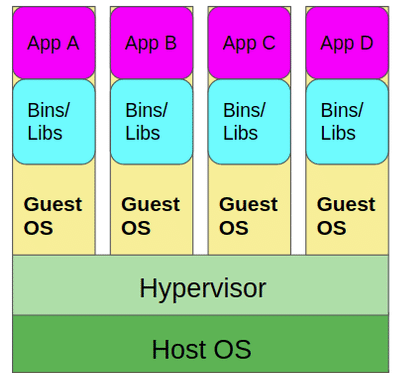
\includegraphics[scale=0.75]{virtualization}
\end{figure}

In days of yore, the only viable way for most companies to work out an IT infrastructure and provision servers for a company was by spending considerable resources on buying physical servers, that is, by spending money on computers and computer parts and running the servers on them. Although it works at first glance, there is an issue that becomes apparent at scale; mismanagement of the machine’s resources, be it its RAM, CPU, or physical memory. In simple terms, two problems could arise; either the company would underspend, and buy fewer physical machines than was necessary, which would lead to recurring outages and stress before new servers could be provisioned to support the ever-increasing amount of users. Another potential disaster could be caused by the company overspending and sinking way more resources into buying and provisioning servers before it was necessary, therefore wasting money that could be used for different purposes.

Ideas of creating some sort of abstraction appeared in the sixties when Jim Rymarczyk from IBM worked out a way to host multiple operating systems on the same piece of hardware, using a hypervisor, which is a software, firmware, or hardware that creates virtual machines, emulations of computer systems running their own operating systems. This type of hypervisor would stand directly above the hardware in the hierarchy, and host multiple virtual machines on top of it. \cite{virtualization}

Later on, at the tail end of the century, a newer virtualization model to provide an abstraction of virtualized resources was developed by the engineers at VMWare. \cite{vmware} It would employ a hosted hypervisor, which means that the hypervisor would be run on a host operating system, making it much easier to manage virtual machines, therefore making virtualization more viable than ever before. \cite{virtualization}

However, VM-based virtualization still effectively “carves out” a part of the hardware resources of the physical server, as it creates a full-fledged operating system that treats its allocated hardware as if it was the only operating system running on it.

With the advent of Docker, container-based virtualization (henceforth referred to as containerization) turned into an extremely popular virtualization technique, which we shall describe in the following chapter. 

\clearpage


\subsection{Containerization}

\begin{figure}[H]
\centering
\caption{Container-based virtualization with Docker \cite{what-container}}
\hspace*{-0.65cm}
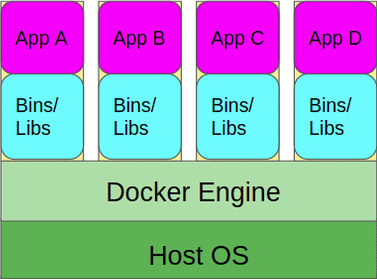
\includegraphics[scale=0.75]{containerization}
\end{figure}

Even though containerization has been around for decades before Docker, for example in the form of BSD “jails”, it is only with the creation of Docker that it truly hit its stride. As seen on the diagrams above, the difference between VM-based and container-based virtualization lies mainly in the fact that while VM-based virtualization creates (virtualizes) an entire operating system, with abstractions for hardware such as virtual CPUs and virtual disks, container-based virtualization uses techniques within the kernel to only virtualize the non-hardware aspects of the operating system, creating a separate root filesystem or network system, while not emulating hardware at all. \cite{virtualization}

This opens up a whole new world of possibilities. Thanks to the efficiency and fast start-up caused by using far fewer resources than full-fledged virtual machines, as well as the opportunity to create truly specialized containers that only focus on providing one service without any redundancies, it’s now possible to manage these containers in such a way that it’s much easier to integrate these services together in a container-based architecture with the added benefit of greater security and easier scaling if each container only has one job.

These containers can then be efficiently managed, upgraded, and be overseen by tools built specifically for the configuration and management of containers, also known as container-orchestration systems, with the most commonly used at the moment being Kubernetes or K8s for short.


\subsection{Orchestration}

As we move into a container-based architecture, in which several microservices delegate tasks and communicate with each other, there arises a need to manage the containers, their lifecycles and the relations between them. This is where the term container orchestration comes in.

There are several tasks which are managed by orchestration tools, such as the provisioning and deployment of containers, health checks of these containers, managing the allocation of resources between these containers and many more. More broadly, orchestration is the automated configuration and coordination of systems and software in general. However, in this particular thesis, we shall focus on container orchestration in particular, that is, on the management of containers. At this moment in time, the most popular container orchestration software by far is Kubernetes, as mentioned in the previous section, however, Docker Swarm is another such tool that posits itself as easier to use, and therefore preferable in certain cases. \cite{docker-orchestration} We shall describe these two platforms and the differences between them in more detail in some of the next sections, as well as a chapter dedicated to Kubernetes.


\subsection{Cloud computing}

Even though the umbrella term "cloud computing" is not directly connected to orchestration, it might be worth it to give an overview here, as there are numerous immediate and powerful benefits of running clusters on the cloud.

As defined by one of the foremost cloud computing corporations in the world, the cloud can simply be described as a collection of servers located all over the world that can be accessed over the Internet, as well as the software and databases that run on those servers. Therefore, by accessing the cloud, users and companies don't need to manage physical servers or run software applications on their own machines. \cite{cloudflare} The rise of cloud computing was revolutionary, as it led to widespread adoption over the years by companies small and large, not at all limited to technology. The staggering upwards trend in the revenue of the cloud computing market over the last few years should serve as sufficient proof. In fact, since 2016, the total cloud market revenue has tripled in value, from around eight billion dollars to a little more than twenty-four. \cite{cloud-market}

In practice, the adoption of cloud computing by companies (or communities) enables the developers to stop worrying about earthly matters like the state of their physical machines, on which the application is running, and allows them to delegate it entirely to the cloud provider. The business model works on a pay-as-you-go approach for every cloud provider that is relevant in today's market, meaning that the customers periodically receive a bill based on criteria such as how much data is stored on the cloud, or how many instances of virtual machines are currently running. \cite{aws-framework} An early adopter, Amazon set the trend with Amazon Web Services in 2006, with Microsoft (Azure) and Google (Google Cloud) following suit. Up to this day, Amazon retains a mammoth share of the total cloud computing market revenue, as well as a huge amount of diverse services, with Microsoft catching up and Google having found its niche in Kubernetes offerings. Currently, all cloud providers are making leaps and strides in maintaining and updating services built specifically for enabling the users to create Kubernetes clusters on the cloud, with Google generally being considered as the best choice, by virtue of it being the main driving force behind the existence of Kubernetes itself.

As for this thesis, a testing cluster was built using Google Cloud and its Google Kubernetes Engine, demonstrating the power of cloud computing in practice. More on this will be revealed in the last chapter.


\section{Technologies}

After explaining some of the theory, let's take a look at some of the most used, tried, and tested containerization and orchestration software nowadays. All of the following tools play a huge role in today's tech world, and it could be said that the advent of microservice-based architecture is largely thanks to these tools. In addition, we will demonstrate a real-world application of these tools in the last chapter, showcasing the Kubernetes cluster made for LearnShell.

\subsection{Docker}

Today, Docker is without any doubt the pre-eminent software for containerization. It was originally meant to be merely an internal PaaS (Platform as a Service) tool for dotCloud, a European company, however, it quickly gained traction as many truly big companies, for example, Microsoft and Google, started noticing the numerous tangible benefits provided by switching to Docker in production. \cite{docker-java} This led to a huge amount of resources being spent on the development and improvement of the Docker project, with several off-shoot tools created as a result, such as Docker Compose, or Docker Swarm.

Even though Docker is a complex piece of software, using it in practice is not as difficult as one may think. Generally, it boils down to writing a configuration file called a Dockerfile. Within the Dockerfile, the user specifies several parameters, such as commands that are to be executed upon deployment of the container, and most importantly, using the FROM keyword, the base image from which the container is to be derived. This image will be downloaded from Dockerhub, which is essentially a public repository of pre-configured images, with minimal overhead. 

Generally, the most commonly used terms in the Docker world are “container” and the aforementioned “image”. An image is an immutable (read-only) file that contains the source code, dependencies, and libraries from which the container is built. On the other hand, a container is a virtualized run-time environment which is created from the image which serves as a template. \cite{docker-phoenix} It is completely isolated from the system on which it runs as well as extremely lightweight in comparison to a virtual machine, mainly due to being virtualized on the application layer instead of the hardware layer of the machine. 

Docker images are stored in registries, which can be either public or private. By running a command inside of the shell, the user can specify an image name as well as a repository and a tag (signifying the version of the wanted image), in order to use that image as a template from which to create a local container. There are numerous repository offerings, that is platforms on which one may host a registry. The most popular by far is DockerHub, however, for purposes such as cloud integration, paid registries can be maintained by cloud providers and other corporations, such as Amazon ECR, Google Cloud Container Registry, or Gitlab Private Registry. Additionally, it is possible (and sometimes preferable) to host a local registry, although it requires additional setting up.

\subsection{Docker Compose}

Not long after its conception, Docker became ubiquitous in software engineering, as it enabled huge projects to be smoothly divided into containers, each doing its own part independent of the other, moving from a monolithic architecture to a microservices-based one. As projects increase in scope, the amount of containers naturally increases as well, and with it the complexity of running them and managing their interactions. For this reason, Docker Compose was developed to be a tool that enables the user to create and start multiple services within their respective containers. All this can be performed by specifying a YAML file, docker-compose.yml, and running it from the command line to deploy a multi-container application. \cite{docker-compose-docs}

In addition, one can specify a bridge network on which the containers defined by Docker Compose may communicate.

\subsection{Docker Swarm}

Bridging the gap between containerization and orchestration, Docker Swarm is, alongside Kubernetes, as of today the most used tool for creating and managing a cluster. It was created as a lightweight, easy-to-use alternative for cluster provisioning, enabling the user to quickly get up to speed and set up a cluster, which is colloquially referred to as “swarm” in the Docker nomenclature. As we have ultimately decided to go for Kubernetes as our technology to create a LearnShell cluster, we shall give a concise description of Docker Swarm in this subsection, followed by a comparison with Kubernetes in the next chapter. However, we shall not delve deep into the details, as this would be beyond the scope of the thesis.

The architecture of a swarm consists of several Docker hosts, that is servers (be it on virtual machines, or physical ones) on which an installation of the Docker engine is present, and one or more containers are running. \cite{swarm-key-concepts} Those are called nodes. There are two, and only two, types of nodes; the manager node and the worker node. The nomenclature is fairly self-explanatory. While the worker nodes only serve as vessels for containers contained therein, the manager nodes, in addition to possessing all the capabilities of worker nodes, also fulfill the function of maintaining the state of the swarm and the communication of its nodes, as well the scheduling of services. In a swarm, a service is a definition of tasks to be executed on a node. \cite{swarm-nodes} For example, one may define a service to be a container created from an image pulled from a registry, which is thereupon provided with a command that is to be executed once the container is up and running. Therefore, when running a swarm and aiming to run a container on a worker node, one should first create the node, and then define a service to run a container on that same node.

In order to allow each node to transfer data between them, a network can be established by using the overlay network driver as well as the bridge network driver. The overlay network driver, also called ingress, handles traffic to a swarm service from outside, while the bridge network driver connects the Docker daemon one host to another Docker daemon on another host. 
Finally, it is worth noting that Docker Swarm plays with other tools in the Docker ecosystem; an example worth mentioning would be Docker Stack, which can be used with a YAML file to quickly deploy a swarm. The structure of this file is extremely similar to a docker-compose.yml file, with minimal differences, such as specifying manager and worker nodes. If we were not using Kubernetes in this project, we would definitely be writing a stack definition file and running it via Docker Stack n order to create a swarm. 

\clearpage

\section{Kubernetes}

In this section, we will dive deep into the inner workings of Kubernetes, our orchestration platform of choice. Due to the sheer depth of the Kubernetes platform, we have dedicated an entire section to this technology. For the reasons why we shall be using Kubernetes in our LearnShell cluster, see the next chapter, specifically the section "Docker Swarm vs Kubernetes". The reader might notice that this section is quite a bit longer than the one dedicated to Docker Swarm; this is not only due to Kubernetes being a more complex piece of software, and also to serve as a sort of glossary to return to from the implementation chapter, which will not be jam-packed with theory.

To quote the official documentation; "Kubernetes, also known as K8s, is an open-source system for automating deployment, scaling, and management of containerized applications". \cite{kube-documentation} We shall be drawing from the documentation quite extensively in this section; where no other sources are provided by citations, we have used the documentation as our source.

\subsection{History}

Kubernetes was developed and launched by many of the same developers that used to work on Borg, Google's internal platform for cluster management. \cite{unix-handbook} These same developers would later work on Omega, which was to be the second generation of Borg, and still an internal, proprietary tool used by Google. Finally, in 2014, the Kubernetes project started in full swing, with the ambition to present an open-source, truly multi-purpose orchestration system, using both the experiences of Google's developers that worked on Borg and Omega years before as well as the power of the open-source community. \cite{medium-kube-history}

The very first version of Kubernetes was released to the public on July 21, 2015, and a partnership with the Cloud Native Computing Foundation was made, boosting development manpower significantly. Later on, in 2016, the first package manager for Kubernetes was released, called Helm, which we shall be using in our cluster, as it is a very powerful addition to the Kubernetes ecosystem. With each passing year, the adoption for Kubernetes is increasing, and this is reflected in the number of commits on Github; based on new commits, its repository was the ninth most popular on Github in 2018. \cite{cncf-kube-graduate}


\subsection{Architecture}

\begin{figure}[H]
\centering
\caption{Architecture of a Kubernetes cluster \cite{kube-components}}
\hspace*{-2cm}
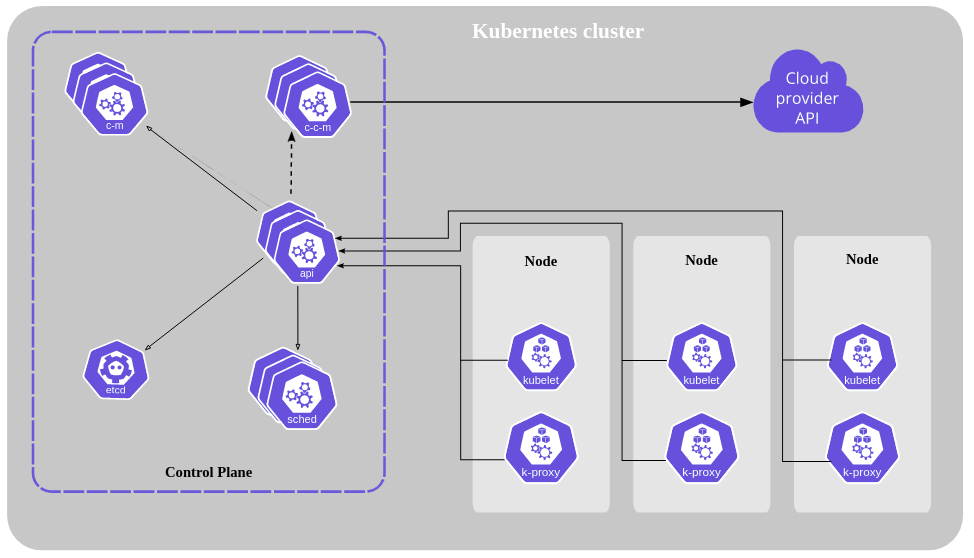
\includegraphics[scale=0.5]{kube-architecture}
\end{figure}

Much like any cluster, a Kubernetes cluster consists of a number of worker machines, referred to as nodes, that run containerized applications within them. One of these nodes has some additional features which enable it to control and manage all the nodes in the cluster; therefore, it was given the name Master. The master node is unique in that it contains a set of applications that is referred to as the Control Plane, which contains the following components:

\begin{itemize}
  \setlength\itemsep{0em}
  \item \textbf{kube-apiserver}, which serves as a front end for the control plane by exposing the Kubernetes API. When we use kubectl during our cluster implementation, we are communicating with that API.
  \item \textbf{kube-scheduler} fulfills the function of assigning newly created Pods (more on them later) and assigning them to nodes. It considers factors such as resource requirements, hardware constraints, and custom configurations made by the cluster administrator. It is one of the key applications in terms of assuring that the cluster is highly available.
  \item \textbf{kube-controller-manager} maintains the controllers of the cluster. A controller is a control loop that constantly watches for any changes in the cluster and changes the state of its workloads to reflect the desired state. A Deployment is an example of a controller that is very relevant to our cluster.
  \item \textbf{etcd} is a highly complex component that stores the current state of our cluster in its entirety as a key-value store. It contains information such as its configuration, specifications, the status of running workloads, network information, and more. \cite{etcd}
  \item \textbf{cloud-controller-manager} is very similar to kube-controller-manager, except it maintains specific to the cloud provider in which the cluster is deployed. If the cluster is deployed on-premises or locally, then the cluster does not have a cloud-controller-manager, as it would be unusable.
\end{itemize}

There are also three important applications that run on every node:

\begin{itemize}
  \setlength\itemsep{0em}
  \item \textbf{kubelet} is an agent that ensures that each containerized application on the node is running on a Pod, and that the Pod is in a healthy state.
  \item \textbf{kube-proxy} allows for network communication between nodes by maintaining specific network rules on each node it is running on.
  \item \textbf{container runtime} is the runtime on which our containerized applications should be running. Currently, the supported container runtimes are containerd, Docker and CRI-O.
\end{itemize}

Now that we have described the architecture of a typical Kubernetes cluster, let us direct our attention toward the basic building blocks of Kubernetes.

\subsection{Building blocks}

The complexity of Kubernetes starts to show in this subsection; there are numerous different resources that one has to be acquainted with in order to create a cluster of some complexity. As a general rule in the Kubernetes community, these resources can be divided into workloads and other types of resources, typically related to the configuration of workloads. A workload can be defined simply as an application running on our cluster at least for some time, somewhat synonymous with the general definition of a microservice. \cite{kube-workloads} In our implementation chapter are some diagrams of the cluster that may shed light on the general relationship between resources.

Let us begin by describing the workloads:

\begin{itemize}
  \setlength\itemsep{0em}
  \item \textbf{Pod} is the smallest deployable resource in Kubernetes. It can be regarded as a wrapper around one or more containers, in which they may share storage and network resources.
  \item \textbf{ReplicaSet} is a controller that ensures that there is a stable set of replica Pods running at a given time, ensuring high availability and fault tolerance. It creates or deletes Pods dynamically to ensure the correct amount of pods is running at any given time.
  \item \textbf{Deployment} in turn serves to provide updates on both ReplicaSets and Pods. In practice, it is recommended to use a Deployment, as it enables the administrator to control everything regarding these resources from one place, from commands to be executed on newly created containers to the number of replica Pods. We shall provide more information on Deployments in the implementation chapter, as we use them for our LearnShell applications.
  \item \textbf{StatefulSet} is very similar to a Deployment, except that it is used specifically for stateful applications, such as databases, by making use of PersistentVolumes or PersistentVolumeClaims as storage units.
  \item \textbf{DaemonSet} is yet another workload that can be mistaken for a Deployment, however, it is different in that it ensures that all nodes run a copy of the pod being managed by it. It has many applications, such as running node monitoring or log collecting applications.
  \item \textbf{Job} creates a Pod and gives it commands to execute until a certain number successfully terminates.
  \item \textbf{CronJob} creates a Pod and gives it commands to execute periodically on a set datetime, written in the Cron format.
\end{itemize}

Now that we have described the workloads, let us continue by listing other resources that are commonly used in Kubernetes (and which shall be used in our cluster as well):

\begin{itemize}
  \setlength\itemsep{0em}
  \item \textbf{Service} provides a way to expose our pods as a network service. The pod can be exposed using a ClusterIP to be accessible only by other applications within the cluster, or either a NodePort or LoadBalancer in order to be accessible from outside as well. Configuring services on our pods is essential in order to assure that network communication within our cluster is not compromised by actions such as redeployments or simply deleting Pods and creating new ones.
  \item \textbf{Ingress} is a rather complex resource that manages external access to services within a cluster. For example, if we want to have a single IP address (and by extension, registered domain) which would access different pods based on the specified path, we would use Ingress to route traffic and provide load balancing for our cluster network by redirecting requests to pod replicas based on routing algorithms.
  \item \textbf{PersistentVolume} and \textbf{PersistentVolumeClaim} are resources that provision a set amount of storage space to be used by certain Pods which are connected to them. This storage space is independent of the space on these pods, which means that if a pod shuts down, it does not lead to data being deleted, as it is saved outside of it. In simple terms, the difference between the two resources lies in that while a PersistentVolume allocates the storage space for use immediately upon its creation, a PersistentVolumeClaim acts as a request for storage, which is executed only when it is needed by looking at our PersistentVolumes and choosing one appropriate for our data. 
  \item \textbf{ConfigMap} and \textbf{Secret} can be regarded simply as collections of key-value pairs to be used by our pods namely as environmental variables. They differ only in that Secrets store encrypted sensitive information, while ConfigMaps do not.
\end{itemize}

While not technically being a resource, \textbf{Namespaces} are a vital part of the Kubernetes ecosystem, and as such should be mentioned. In short, Namespaces fulfill the function of separating virtual clusters backed by the same physical cluster. This means that we can run multiple different clusters on the cloud or on-premises, and use namespaces to isolate them from one another. This is helpful especially in large organizations, but best practices dictate that each cluster should have its own separate namespace. In our project, this would be the "learnshell" Namespace, and we shall make it so.

\subsection{Authentication and authorization}

While this topic is particularly complex, a brief overview will be provided as authentication and authorization are important parts of any cluster, including ours.

In Kubernetes, there are two categories of users: normal users, and ServiceAccounts created and managed by the cluster. While there are numerous ways for users to authenticate and be able to make API calls to the api-server, we shall focus on service accounts here, as they are of particular importance in our implementation of a CI/CD process. A \textbf{ServiceAccount} is a special type of account that can be used by Pods to contact the api-server just like a normal user would. This can be useful in many cases, such as when we want to restart a Deployment on cue, for example as part of our CI/CD pipeline. Each ServiceAccount in our cluster has a unique bearer token with which it can authenticate to the api-server to execute commands via API calls.

However, before actually execute these commands in practice, the api-server first checks if the ServiceAccount in question has sufficient authority to perform them. For this, \textbf{Roles} and \textbf{RoleBindings} are used. The administrator can create a role with specific authority, for example restarting Deployments, and bind this role via a RoleBinding to the ServiceAccount of a specific pod. Once that is finished, the pod can perform API calls to the api-server of the cluster, and the api-server will execute these calls after confirming that the ServiceAccount is correctly authorized.


\chapter{LearnShell Cluster Analysis}

In this chapter, which is the first of the two that describe the practical part of this thesis, we shall explain our architectural decisions as well as the motives behind them. We will describe the technologies used and why they were necessary, and where need be, we shall compare the most viable technologies for our particular use case.

\clearpage

\section{Docker Swarm vs. Kubernetes}

Since we will be implementing a cluster for LearnShell, one of the most important decisions we had to reach was to make an informed choice between Docker Swarm and Kubernetes as our orchestration platforms. Therefore, in this section, a comparison of Docker Swarm and Kubernetes will be made; for each platform, we shall describe the general use cases, the advantages, and disadvantages, as well as their future in the industry. Then, we will concentrate on LearnShell specifically, and reach a final decision on which platform is the best for our use case in particular.

\subsection{General comparison}

As we have already discussed, the main practical difference between Docker Swarm and Kubernetes historically lied in their complexity. Docker Swarm is much more tied to Docker itself than Kubernetes, which supports several container runtimes. In fact, as of 2021, the default container runtime of the latest Kubernetes version is containerd. \cite{kube-containerd} In fact, swarm mode is natively included in Docker, so there's no need to install additional packages. As for Kubernetes, things aren't so simple, as we will elaborate later. 

Additionally, the learning curve is much steeper with Kubernetes, however, Kubernetes has a much, much more rich ecosystem, and as such there are many problems that can be easier to solve with Kubernetes than with Docker Swarm. Regardless of the learning curve of each platform, it has to be said that the documentation of both platforms is impeccably written, even though the author of this thesis finds that Kubernetes has an edge in this regard. One strength, in particular, is the option of running a test cluster via an in-browser terminal, connecting to the cloud via SSH. This enables the user to immediately apply in practice what was learned through reading the documentation. Therefore, it could be said in summary that while Docker Swarm is easier to grasp initially, both platforms have great documentation that explains the concepts quite capably, with Kubernetes being slightly better.

One area where Kubernetes has a clear, unassailable advantage is industry adoption. As proof, taking a look at the respective Github repositories of each platform should suffice (this is possible due to both platforms being open-source from the very start, and as such, all the code is publicly available). By glancing at the pull requests of each repository (in layman's terms, a pull request is a request for review of code before it is merged into a branch of a repository, and therefore integrated into the codebase), one can see that there is a world of difference; currently, the amount of pull requests for Kubernetes is ten times more than the amount for Docker Swarm. \cite{swarm-pull, kube-pull} Another important factor is that Kubernetes was initially developed, and is being maintained largely by Google; an industry behemoth. This means that there is a near-infinite reserve of resources dedicated to keeping Kubernetes alive and well.

Industry adoption spills over to many other factors, one of them being third-party support for a given orchestration platform. In this, Kubernetes is a clear winner. Each major cloud provider maintains a service designed specifically to simplify the creation of a cluster on the cloud, with Google Cloud naturally being the fan favorite, due to its close connection to the product. In addition to that, foremost git-repository managers provide integration with Kubernetes, facilitating the integration of the cluster into the DevOps lifecycle of the given project.

One notable factor that should not be underestimated, and is again tied to industry adoption, is the future of each platform. Kubernetes is currently extremely dominant in the orchestration space, and as such, it is entirely possible that within the next few years, support for Docker Swarm could be dropped completely. The developer should take this into account, especially when it concerns any projects that should be here to stay, as migrating a large project from Docker Swarm to Kubernetes could be a challenging feat.

In summary; the strength of Docker Swarm lies in its shallow learning curve, as well as its seamless integration with other Docker offerings. However, Kubernetes wins in every other category; it is feature-rich, exquisitely documented, and appears to be extremely dominant in comparison to Docker Swarm in the industry.

\subsection{Project-specific comparison}

Finally, it is time to consider our options specifically regarding LearnShell, and choose the best orchestration platform for our use case. We shall decide based on these criteria; ease of setting up a cluster, maintainability, versatility, and integration with other services used by LearnShell.

When it comes to quickly setting up a cluster, Docker Swarm wins; its natural integration with other Docker services, such as Docker Compose, comes in really handy, as it allows us to run a few commands to get a cluster (or swarm, to adhere to the nomenclature) running. However, the rich ecosystem of Kubernetes holds its own here, as it gives us several options, such as Minikube or Kubernetes-in-Docker, to quickly set up a cluster. Nevertheless, a minimal understanding of how Kubernetes works is still necessary, and as such, it remains true that a little more time reading the documentation will be necessary.

In the case of LearnShell, we define maintainability by the difficulty of keeping the cluster up and running, as well as updating the containers within and adding new ones without disrupting it. Another important factor is how difficult it would be for new members of the LearnShell team to get up to speed with the cluster. In this case, the sheer size of the Kubernetes ecosystem plays a very important role, since any potential new developers have a plethora of articles, videos, books, or documentation on the internet at their disposal, while Docker Swarm is dwindling in its presence. Therefore, one can assume that if the cluster were to be improved upon in the future, it would be far easier to do so with Kubernetes, since it is certain to be a dominant player in the orchestration world for some time.

Versatility is admittedly a rather broad term to apply here, but in this case, we are addressing questions such as how difficult it would be for us to change up the proxy server on which LearnShell is running, or the database used by LearnShell, or (most importantly) how easy or hard it would be to migrate the cluster from on-premises architecture to the cloud. Whereas the services used by the cluster are quite easy to change up in both platforms, since Docker Swarm with its natural integration of Docker containers allows us to simply pull a different image if we wanted to use a different database engine, for example, and Helm makes this trivial with Kubernetes as well, it is the cloud where Kubernetes really shines here. Since there are comprehensive offerings on the cloud for Kubernetes, such as GKE on Google Cloud, it is entirely within the realms of possibility to migrate the entire cluster to the cloud. This could potentially not only lead to less upkeep, but to a much smoother experience of maintaining the cluster, especially now that GKE Autopilot was introduced, which promises greater optimization of resource use by the cluster, leading to greater performance in addition to lower costs of upkeep. \cite{autopilot}

The last criterion would be the integration with other services, which essentially points to future possibilities of running a continuous integration routine on Gitlab (where LearnShell repositories are hosted), in which it would be possible to automatically replace older versions of containers with new ones or possibly keeping different clusters for different purposes, such as a staging cluster for testing purposes, and a production cluster, which the students and teachers would be using. In this, Kubernetes is a clear winner, as Gitlab is making a great effort in being containerization and orchestration friendly by allowing even free-tier users to integrate a cluster with their projects. \cite{gitlab-kube} Also, it coincidentally allows us to keep a private container registry for free, and creating CI routines with Gitlab Runners. However, unfortunately, for the purposes of LearnShell, there are only so many features that we can use at this moment in time, since the current release of Gitlab (11.8.10.) used by the university is more than two years old, and we are using the Community edition, which doesn't have some features that could prove very useful. Among these features is the Kubernetes Agent or Auto DevOps, a platform that advertises reduced complexity in setting up pipelines, and probably most importantly in our case, the option to integrate multiple clusters into Gitlab, which would give us the option to have different pipelines, for example, one for testing purposes, and one for the production cluster. Nevertheless, the option to use a private Gitlab registry remains available, as well as the option to use Gitlab Runners on our cluster to run CI pipelines; we shall elaborate on this later.

After much deliberation, we have decided to choose Kubernetes as our orchestration platform of choice. Even though the learning curve is undoubtedly quite a bit steeper than the alternative, what gives it its edge in the case of LearnShell is the fact that continuous integration routines for the cluster are natively available within Gitlab, and that there is a strong argument for potentially migrating the cluster from on-premises to the cloud, as all the cloud providers are actively working on making this as painless as possible. Also, the industry adoption of Kubernetes leads to a great amount of resources being available in the case of troubleshooting the cluster.

\section{On-premises vs Cloud}

This section is dedicated to comparing the viability of hosting the LearnShell cluster on "bare metal" servers potentially provided by the university with hosting it entirely on the cloud, here represented specifically by GCP.

In the industry, Kubernetes clusters are almost never used on-premises. There are several reasons for this, with the main ones being:

\begin{itemize}
  \setlength\itemsep{0em}
  \item Potential hardware limitations
  \item Potential for unrecoverable disasters
  \item Exponential difficulty of maintenance of the cluster
\end{itemize}

The first two reasons are quite self-explanatory; if a cluster is deployed on-premises, there's always a chance that somewhere in the process, it is found out that more resources are needed for it to be highly available, which can be a problem if we can't allocate more resources on our current setup. Also, there's always a chance of a disaster happening on the hardware level; even though a Kubernetes cluster, if correctly set up, is immune from failures based on one part of the application crashing, it still needs to be run on hardware. Therefore, if a disaster such as a server room fire occurs, the consequences for the cluster would be absolutely dire.

However, the most extensive disadvantage is the fact that an on-premises cluster would need to be carefully maintained in order to function at its best. One would have to consistently manage updates, security, backing up of persistent data manually, which could lead to hours upon hours of time spent on the maintenance of the application. This could be a problem especially in the case of organizations that have high turnover, and therefore the cluster would potentially be maintained by someone who played little part in setting it up.

All of these problems can be resolved by using a cloud provider, such as Google Cloud, for hosting the cluster; hardware resources of data centers are practically boundless, and even in the case of an absolute blackout in the region, the cluster would be promptly moved to machines in another region. In addition, by using managed Kubernetes services, one can avoid all the headache of ensuring periodic back-ups of databases or adhering to best orchestration practices, be it in matters of security or keeping updates up to date, as the cloud provider would handle all this automatically on its own. \cite{cloud-native-kube}

There is one notable fact that should be called attention to; Kubernetes can be built rather easily to be as provider-independent as possible, and therefore it is viable to host a cluster on any cloud provider, as well as on-premises with minimal changes to the configuration files in which the cluster is to be defined. As such, our practical solution, which is in the following chapter, is made to be completely identical for both the on-premises cluster as well as for the cloud cluster. 
With that in mind, we can easily move between an on-premises cluster and a cloud-hosted one, depending on the direction LearnShell goes in. For example, it could be prudent to run a staging cluster for testing purposes on a school server, with the added bonus of running our CI/CD-focused deployments there, as those do not depend on performance in our use case at all. On the other hand, to maximize performance, a production cluster should ideally be run on the cloud, as a cloud-based solution would be infinitely scalable and immune to complete disasters such as a server room fire on-premises. 

\section{Package manager}

During the process of writing code, software developers may often encounter problems which are better solved by using tried and tested libraries instead of writing the code by themselves. This can have two advantages; spending less developer time and providing the developer with secure and well-architected code (provided that he chooses a library of good quality). Today, to install these libraries, one would use a package manager, that is a system that automates the process of installing and updating libraries, among other features. In LearnShell, for example, npm is used for the JavaScript front-end, and pip3 is used for the Python back end.

In the Kubernetes world, a package manager of sorts exists as well; its name is Helm, and it manages packages called \textbf{Helm charts}, which are simply bundles of configuration and definition files to create Kubernetes workloads and resources. By taking a closer look at the Docker containers currently employed in LearnShell, we quickly notice that the PostgreSQL and Redis containers have no additional configuration, aside from environment variables and port mapping. In addition, as we have outlined in the Kubernetes section of the previous chapter, databases can be a bit more verbose to set up, as they represent a stateful component of an application; therefore, after a database pod is killed and revived, there should be a persistent layer on which the data remains. Also, if we run multiple database pods, all of these pods should always be connected to the same persistent volume. In practice, we would need to set up a StatefulSet, a PersistentVolume, or a PersistentVolumeClaim and expose the database on a headless Service, which is a considerable amount of manual configuration.
In summary, using Helm is very appropriate in situations where we know that we may be reinventing the wheel by writing multiple configuration files and commands. Additionally, by using Helm charts that abide by the current best practices of cluster configuration, we avoid the potential headache of improper configuration, or one which does not adhere to the best practices; however, we should still be careful on which Helm charts to trust.

To make use of Helm charts, one first has to add a repository from which to pull these charts. Afterwards, by using the install command, helm checks the currently added repositories for the chart and installs the chart if it is found, giving it the chosen name. An instance of a chart running on Kubernetes is referred to as a "release"; by signifying a name in the install command, all the workloads and resources in the cluster that are part of the release will be called as such. Importantly, a YAML file, usually called \verb|values.yaml| (in our case, we shall prefix it by the name of the release) can be referred to from which variables can be pulled to customize the configuration of the release, such as login credentials, disk space allocated by the persistent volumes, or static IP addresses from which to access the cluster from the internet in the case of charts focused on networking. This file is called a Values file in the Helm nomenclature. \cite{using-helm}

In addition, there are several other tricky aspects than just stateful application which can be handled by using Helm. For example, as we will demonstrate, charts can be used to simplify network configuration, and to set up CI/CD with internal access to the cluster, which can prove extremely useful for our particular use case.


\section{Private container registry}

For our cluster to run Deployments, we need to provide Kubernetes with the necessary Docker images from which to create containers contained within the Pods maintained by these Deployments. For that, there is a requirement for a private container registry, wherein these images will be located. From our research of possible private container registry offerings, we have arrived at a crossroads between three alternatives:

\begin{itemize}
  \setlength\itemsep{0em}
  \item Self-hosted registry
  \item Google Container Registry
  \item Gitlab Container Registry
\end{itemize}

Since we have deployed a cluster on Google Cloud, a natural option would be to also host our images there; it would enable easy and robust integration with our GKE-hosted Kubernetes cluster. However, there is a monthly fee of 0.026 dollars per GB per month, and we would like to avoid any monthly payments as much as possible. \cite{gcr-pricing} Therefore, we shall narrow our scope to free offerings. Out of those, we have only found two possibilities that are both free of charge as well as private. We could use a self-hosted registry, which is definitely possible. However, there are two disadvantages; since it is self-hosted, we would have to set it up, as well as maintain it manually, which could lead to trouble down the road, as we are trying to maximize automation, and therefore avoid the need for manual maintenance. Secondly, such a solution would be harder to integrate with Gitlab and its CI/CD offering; it would still be possible, but additional configuration would be necessary, increasing complexity. There is only one option that is both free, private and enables integration with Gitlab, and that is hosting the image registry on Gitlab itself, using the Gitlab Container Registry. This is also the best provider-independent option, as a DevOps pipeline on Gitlab would be easiest to improve upon by hosting the images there, as well.

As such, we arrive at the conclusion that Gitlab would be the ideal option for a private container registry, especially when taking proper CI/CD routines into consideration.

\clearpage

\section{Continuous integration and continuous deployment}

\begin{figure}[H]
\centering
\caption{Visualization of typical CI/CD pipelines \cite{cicd-diagram}}
\hspace*{-2cm}
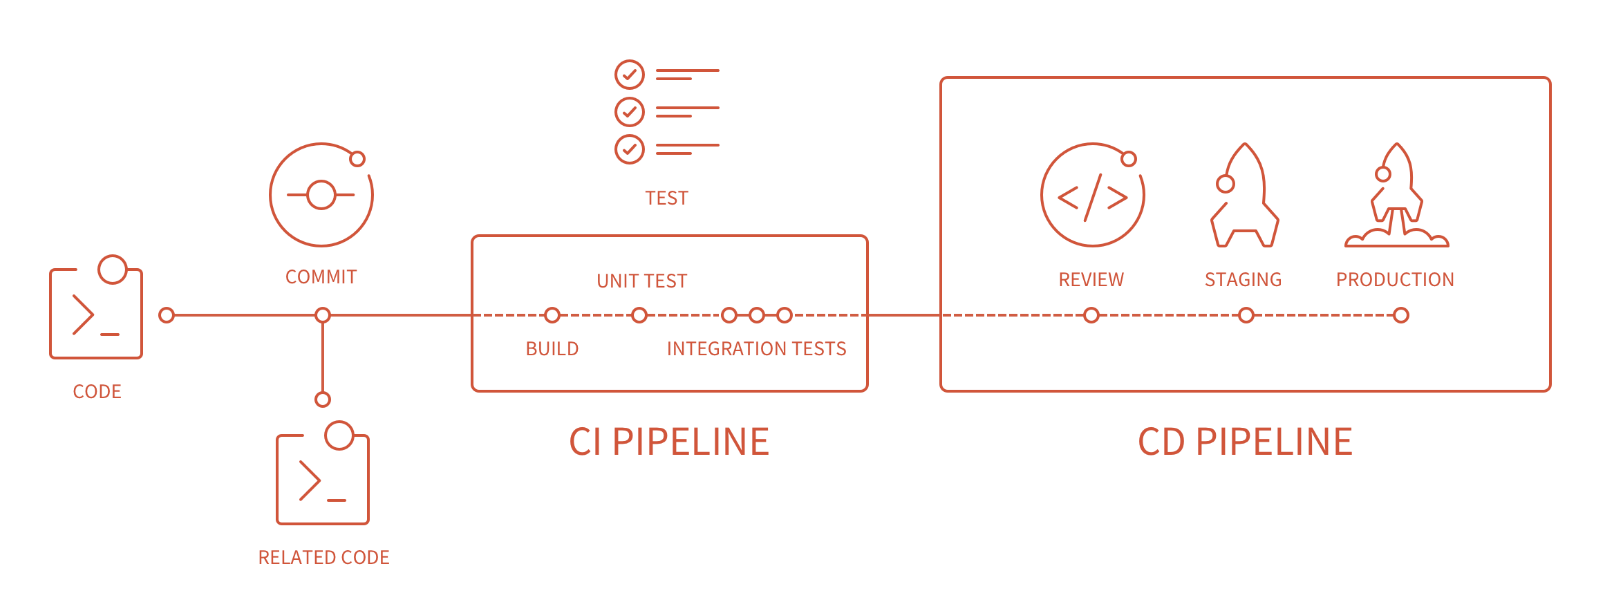
\includegraphics[scale=0.3]{cicd}
\end{figure}

As the last goal of this thesis, we would like to implement a basic CI/CD configuration for LearnShell. To do this, we were requested to use the tools made available by Gitlab, the Git-repository management platform used by our university. Therefore, the choice of software used for CI/CD was essentially made for us; although, we are perfectly in agreement with that choice, as Gitlab CI has all the features we need.

First, let us quickly describe what the terms CI/CD actually mean;

\begin{itemize}
  \setlength\itemsep{0em}
  \item \textbf{Continuous integration} is the practice of building and testing applications continuously and automatically; in practice, this would generally mean that every time a new commit is pushed into a Git repository, a dedicated server, usually called a build server, would execute jobs that would be comprised of building the application and running tests on it in order to verify if the newly built version is working correctly.
  \item \textbf{Continous deployment} is another step beyond CI; if we can build and test our applications continuously, there's no reason not to automate deployment as well, which is where CD comes in; upon building and testing our application, the application can be deployed into either our staging server or our production server, or both. \cite{cd-guide}
\end{itemize}
 

In order to properly analyze the technologies which we shall be making use of to enable proper CI/CD pipelines, we should take care to accurately define our goals in a diagram.

\begin{figure}[H]
\centering
\caption{LearnShell CI/CD pipeline}
\hspace*{-3.6cm}
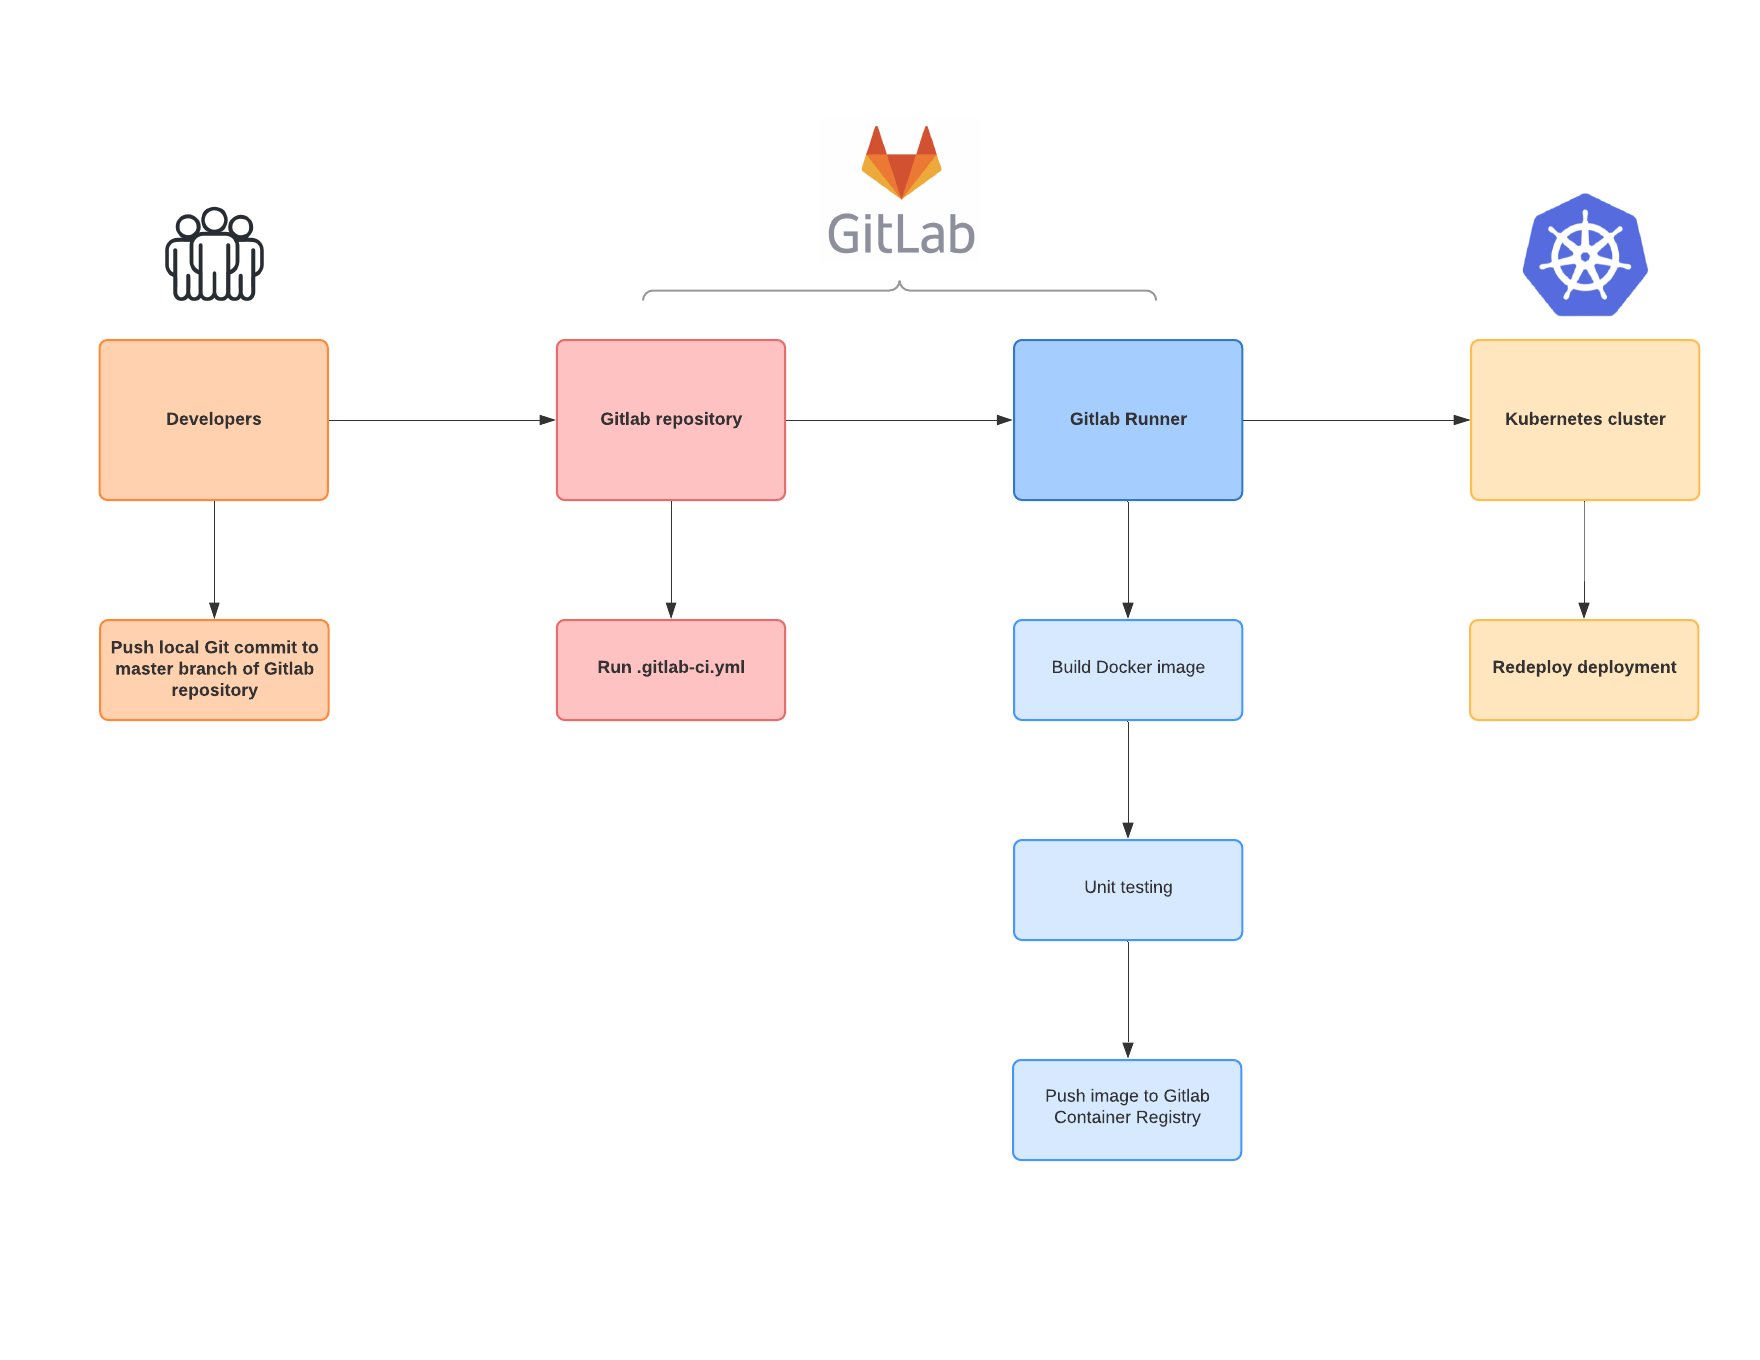
\includegraphics[scale=0.7]{learnshell-cicd}
\end{figure}

In this diagram, the uppermost large rectangles represent the parties performing certain tasks and the smaller rectangles below them represent their assigned tasks, performed sequentially. To sum it up, we would like to do the following on each push to the master branch of a LearnShell Gitlab repository:

\begin{enumerate}
  \setlength\itemsep{0em}
  \item Build a Docker image(s).
  \item Run unit tests if any are written.
  \item Push the local images to our registry.
  \item Redeploy Deployment inside our Kubernetes cluster containing the Pod which pulls the freshly pushed image.
\end{enumerate}

To build a pipeline running these tasks, we shall be using Gitlab CI/CD. To achieve this, we shall be writing a .gitlab-ci.yml file, which will be parsed to create a pipeline on every new commit into the repository. And to run the tasks (or to adhere to the Gitlab CI terminology, jobs), we shall make use of Gitlab Runner, which is an application that serves as a platform for running jobs specified in that Gitlab pipeline. More details regarding the implementation of our pipelines will be provided in the next chapter.



\chapter{LearnShell Cluster Implementation}

In this final chapter of our thesis, we shall focus completely on the practical side, which is the implementation of our cluster in practice. An overview of our code and our directory structure is to be provided, as well as diagrams showing the cluster in its entirety. However, be advised that we will not be going deep into theory since that was already elaborated upon in the previous chapters.

Importantly, the cluster which we shall be focusing on in this chapter is the one running on Google Cloud, however, there is no difference between the on-premises cluster implementation and the cloud one; this is merely the personal preference of the author, as the user interface of Google Cloud proves to be really helpful for debugging. Lastly, one may notice that our cluster implementation does not contain the LearnShell evaluator. This is because the evaluator has not yet been containerized to issues outlined in the first chapter. Once a containerized evaluator is implemented, it is not at all difficult to include it in our cluster. As of right now, however, the cluster can work with the evaluator server instead, although some additional configuration may or may not be needed.

\clearpage

\section{Technologies}

To start off, let us briefly summarize the main technologies we have made use of after our analysis:

\begin{itemize}
  \setlength\itemsep{0em}
  \item \textbf{Kubernetes} as our orchestration platform.
  \item \textbf{Docker} as our containerization platform.
  \item \textbf{Gitlab Container Registry} as our private container registry.
  \item \textbf{Helm} as our package manager.
  \item \textbf{Google Cloud} as our cloud platform, and by extension \textbf{GKE} as our Kubernetes engine.
  \item \textbf{Minikube} as our local development single-node cluster platform.
  \item \textbf{Gitlab CI/CD} and \textbf{Gitlab Runners} to facilitate CI/CD for LearnShell components.
\end{itemize}

As a side note, we have used Linux as our operating system of choice both locally and on the cloud, due to its seamless integration with Docker. On Google Cloud, we have deployed three VMs running Debian, as it is the distribution we are most familiar with. These VMs were provisioned automatically by GKE to function as nodes for our cluster. As for the on-premises, implementation, we are currently running it on Minikube; however, a Minikube cluster is not quite fit for production, since it is only a single-node cluster tailor-made for local development. On the other hand, hosting a cluster on the cloud makes it far more viable for production right off the bat, as we have the option of adding and removing nodes as we see fit (alongside lots of other features), and as such we can create a cluster optimized for high-availability, allowing for drastic performance improvements by utilizing resources of multiple machines (or nodes, in the Kubernetes nomenclature) as well as protecting us from disasters such as node crashes by having other nodes step in before the crashed node recovers. \cite{high-availability}

Less importantly,  Vim was used as our text editor due to its ease of use when editing configuration files and availability on machines on the cloud. Also, we have used Bash in our build script for its prevalence in the Linux world.


\section{Project structure}

Let us continue with a brief overview of the project structure of the repository with our cluster configuration.

\begin{figure}[H]
\caption{Directory tree of the LearnShell Cluster project}
\hspace*{3.5cm}
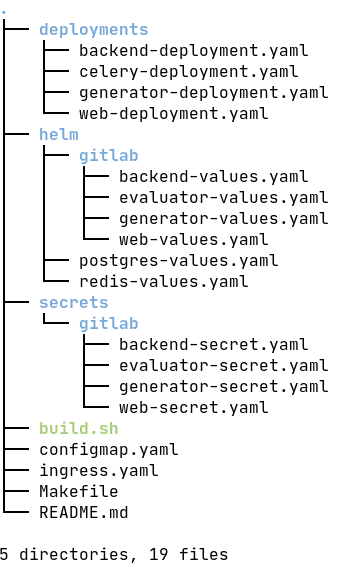
\includegraphics[scale=0.5]{tree}
\end{figure}


As we can see from the output of running \verb|tree| in the project root, the files in our repository are almost exclusively either YAML configuration files or shell scripts, which is par for the course in a Kubernetes application; the YAML files contain instructions based on which we build all resources in our cluster, while the shell script uses them to build our cluster from scratch. By running \verb|wc -l| on all the (not auto-generated) files in the repository, we arrive at an estimation of a little less than 350 lines of code, with the bulk of it being in the Deployment configurations and the shell script.

There are several facts worth mentioning regarding our project structure. Firstly, as one can see from the first figure, there are no files specifying different configurations for specific cloud providers (or for on-premises clusters). This is because with some additional work and research regarding matters such as backward-compatible versions of Ingress, Kubernetes allows us to create truly provider-independent cluster configurations; therefore, as of right now, we can build our cluster using the build script on both Google Cloud as well as on-premises, and there is no particular reason to doubt that it would be the same for other cloud providers, such as AWS or Microsoft Azure. Secondly, the project might seem deceptively small, especially when one considers the number of lines written. We achieved this by making use of two tools; Helm charts to forego having to write configuration files for our databases as well as using shell commands (such as \verb|kubectl expose deployment| to create services) instead of specifying our workloads and resources in YAML files. 

Should we instead decide to build Roles, ServiceAccounts, PersistentVolumeClaims, StatefulSets, etc. via \verb|kubectl apply| on configuration files, our project would quickly increase in size, if we go purely by the number of lines of code. This would not be advantageous, not even for configuration debugging purposes, since kubectl has commands specifically for describing workload and resource specifications and reading logs of workloads.

\section{Functionality}

Before we get to any diagrams, we should properly explain what the project does. Essentially, it all boils down to our Makefile and build script. By calling \verb|make|, a cluster is built from scratch in the "learnshell" namespace, in order to isolate the workloads and resources of our cluster from those potentially running on the user's machine(s) for other purposes. 

However, there are some prerequisites for our build script to run correctly. Obviously, Kubernetes should be installed on the machine, as well as its prerequisite, Docker. Next, Helm is required for installing Helm charts, which play a very significant role. Also, a shell interpreter is required for the build script to run, and Make should be installed to call Makefile commands. However, one can also run the build script by itself; the Makefile is there merely for the convenience of the user. Finally, a platform to run the cluster on is required; the script is verified to work on Minikube and GKE, however, it should work everywhere, even though we have not tested it on other providers.

Upon running the Makefile command, setting up the cluster could take several minutes; be advised that the process is far slower on the on-premises cluster, due to it running on Minikube, which is a single-node cluster. In comparison, the Google Cloud cluster uses GKE to make sure all the pre-provisioned nodes share the load of setting it up and maintaining it and is therefore many times faster.

\subsection{Documentation}

For an exhaustive guide on how to set up the LearnShell cluster, see the Markdown documentation packaged with the project in the Gitlab repository of the cluster. The documentation includes a step-by-step guide as well as a list of current issues and potential improvements.

\section{Build script in-depth}

To properly understand the process of building a cluster from the ground up, let us through the key sections of our build script. To do this, we shall analyze what is happening inside when specific Makefile tasks are executed.

\subsection{make help}

\begin{figure}[H]
\centering
\hspace*{-0.5cm}
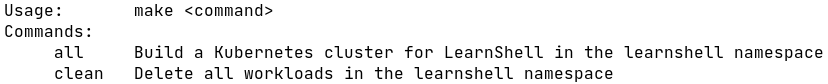
\includegraphics[scale=0.5]{build-help}
\end{figure}

By far the simplest of the three, \verb|make help| merely outputs a list of commands that can be called.

\subsection{make clean}

\begin{figure}[H]
\centering
\hspace*{-0.5cm}
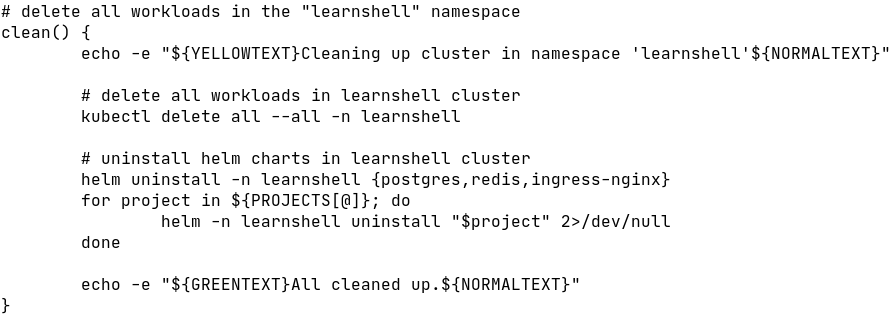
\includegraphics[scale=0.5]{build-clean}
\end{figure}

Moving on, the \verb|make clean| task deletes all workloads in the "learnshell" namespace, which is the reserved namespace of our cluster. It does so by calling \verb|./build.sh clean|, which in turn calls the function described above and exits immediately. The code itself is rather self-explanatory; first, we delete all workloads within the cluster, then we uninstall our Helm charts in order to be able to reinstall them completely in the future.

This function serves another important role, as we have configured our build script to call it every time an error occurs within the creation of the cluster. The advantage of this is that there are no side effects related to workloads in case of failures during the build process, and one can call the build script without worrying about polluting the namespace in case of any complications.

\subsection{make}

\begin{figure}[H]
\centering
\hspace*{-0.5cm}
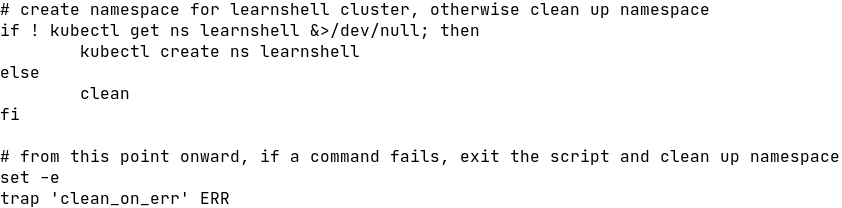
\includegraphics[scale=0.5]{build-namespace}
\end{figure}

Finally, we arrive at the most important task, which is building the cluster. This is done by simply calling \verb|make| without any additional arguments, which executes our build script in full. 

As a preliminary stage, the script pre-emptively ensures that we have a clean "learnshell" namespace to work with. Afterwards, the script is configured to immediately exit in case of any errors, and just before exiting, to clean up the namespace and echo an error message.

\begin{figure}[H]
\centering
\hspace*{-1.5cm}
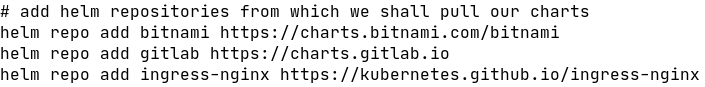
\includegraphics[scale=0.5]{build-helm1}
\end{figure}

\begin{figure}[H]
\centering
\hspace*{-0.5cm}
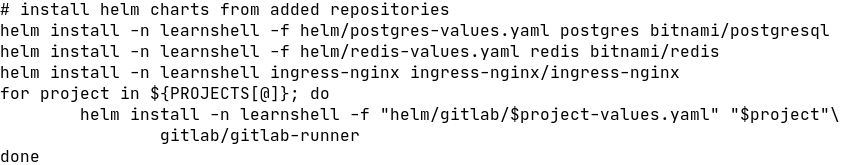
\includegraphics[scale=0.5]{build-helm2}
\end{figure}

Next, the script makes sure that we have the correct Helm repositories on hand, and installs the necessary Helm charts while updating them with our custom values. The PROJECTS variable refers to the different LearnShell projects on Gitlab, in this case, web (the front end), core (the backend), generator, and evaluator. Therefore, we create Gitlab runners for each project, pre-emptively even for the evaluator, as it can potentially benefit from CI/CD even without being containerized at the moment, for example, to potentially run unit tests on each commit.

\begin{figure}[H]
\centering
\hspace*{-1.5cm}
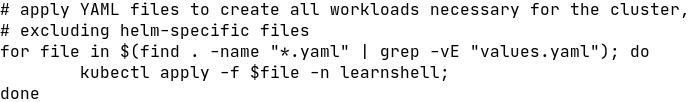
\includegraphics[scale=0.5]{build-kube1}
\end{figure}

Here, we traverse our work directory and create Kubernetes resources where possible, while omitting Helm-related files. 

\begin{figure}[H]
\centering
\hspace*{-0.5cm}
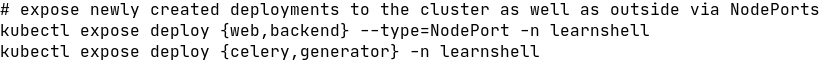
\includegraphics[scale=0.5]{build-kube2}
\end{figure}

After creating our resources, we expose all LearnShell Deployments. Since we are planning to make the front end as well as the back end accessible by the end-user, we expose them via NodePorts, while keeping other services exposed only within the bounds of our cluster. More on this will be revealed in the Networking section.

\begin{figure}[H]
\centering
\hspace*{-0.5cm}
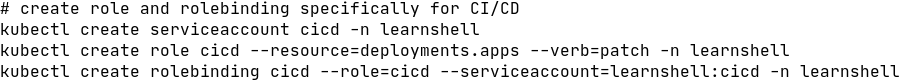
\includegraphics[scale=0.5]{build-kube3}
\end{figure}

This final part of our build script is related to the CI/CD process. A ServiceAccount is generated that only has one privilege, which is updating Deployments. All our Gitlab Runners will make use of this account to facilitate continuous deployment within our cluster.

\section{Deployments}

After the build process is finished, we are presented with a complete cluster, including diverse Kubernetes resources such as Deployments (and by extension ReplicaSets, Pods), StatefulSets, PersistentVolumes, PersistentVolumeClaims, Services, ServiceAccounts, Secrets, ConfigMaps, and more. This section in particular is dedicated to the Deployments which in our case specifically represent components unique to LearnShell.

\begin{figure}[H]
\centering
\caption{Deployments within our cluster}
\hspace*{-2cm}
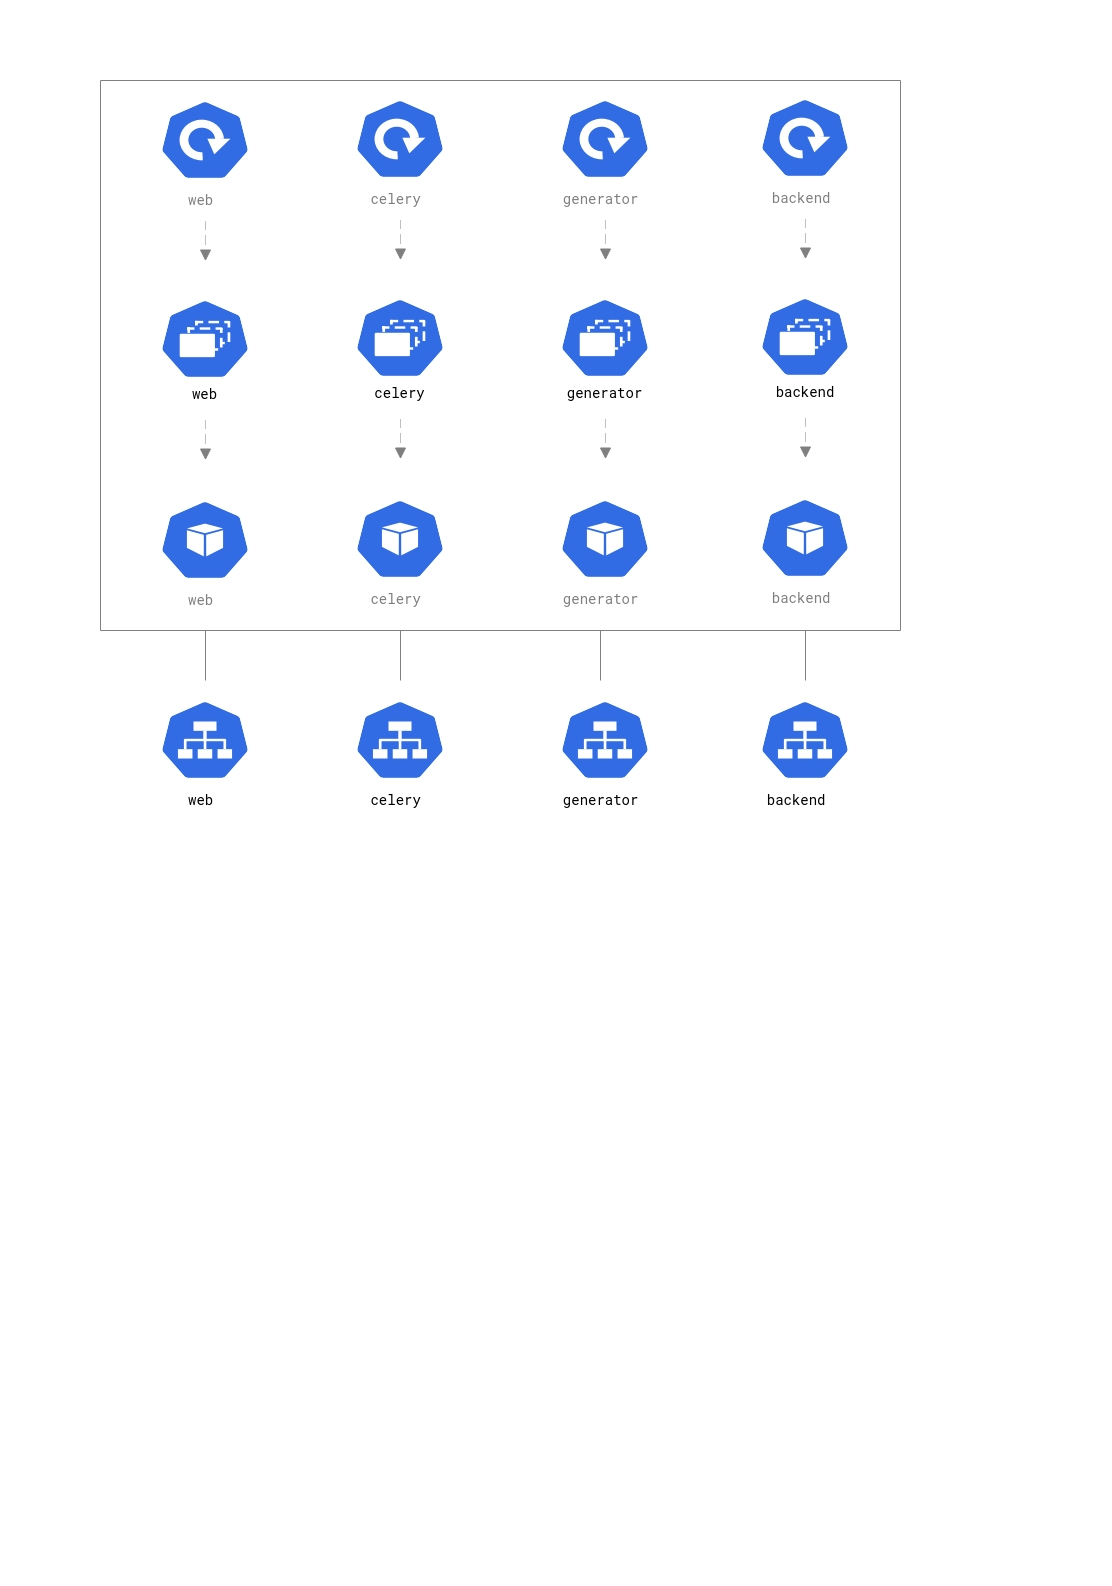
\includegraphics[scale=0.5]{deployment-diagram}
\end{figure}

As we can see in figure 4.2, we have four LearnShell Deployments in total, named respectively web, celery, generator, and backend.

The general workflow of each of our Deployments is as follows:

\begin{enumerate}
  \setlength\itemsep{0em}
  \item \textbf{Deployment} resources are generated by using \verb|kubectl apply -f| on our YAML file containing the Deployment definition.
  \item \textbf{ReplicaSet} resources are in turn created and maintained by our Deployments.
  \item \textbf{Pod} resources are created, updated, and deleted by our ReplicaSets, according to the data specified in our YAML file; of particular importance is information such as the number of replica Pods that should be running at any given time, the ports on which our Pods shall communicate or the images from which our containers should be created.
\end{enumerate}

In addition, each of our Deployments is exposed to our cluster via its own Service to assure seamless communication between the Pods maintained by them.

\subsection{Deployment configuration}

To provide some insight into our Deployments, let us take a closer look at one of our YAML files in which they are specified. For this purpose, we shall be using our backend Deployment.

\begin{figure}[H]
\centering
\hspace*{-0.5cm}
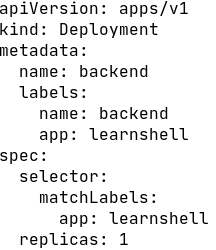
\includegraphics[scale=0.5]{deploy-backend1}
\end{figure}

In each Kubernetes object definition, there are four required fields:

\begin{itemize}
  \setlength\itemsep{0em}
  \item \textbf{apiVersion}, which defines the version of the Kubernetes API that we want to use to create our object. By specifying apps/v1, we tell the Kubernetes engine to use the latest version.
  \item \textbf{kind} specifies the object to be created; in our case, a Deployment.
  \item \textbf{metadata} contains data that help us uniquely identify our object. Typically, that would be a name, labels of all kinds, such as the application to which the object belongs, or the namespace. Here we use just two labels; one for the name of our resource, and the second for our application.
  \item \textbf{spec} is the most verbose, as it entails the state which is desired for our object. As such, the spec field is very different across objects, with very different specifications between different resources. In the next snippet, we shall go into more detail regarding our spec field.
\end{itemize}

Importantly, within the spec field, the \textbf{replicas} keyword commands the ReplicaSet created by our Deployment to create (and maintain) as many replica Pods as we want. In our case, just one, as this cluster is not in production. However, a production-ready cluster would have as many replica Pods as is necessary to ensure high availability between them. Furthermore, the \textbf{selector} field serves as a way for our resources to identify each other; here, we specify that the Deployment should be matched to other resources that also have the learnshell app label, therefore grouping them together via this label.

\begin{figure}[H]
\centering
\hspace*{-0.5cm}
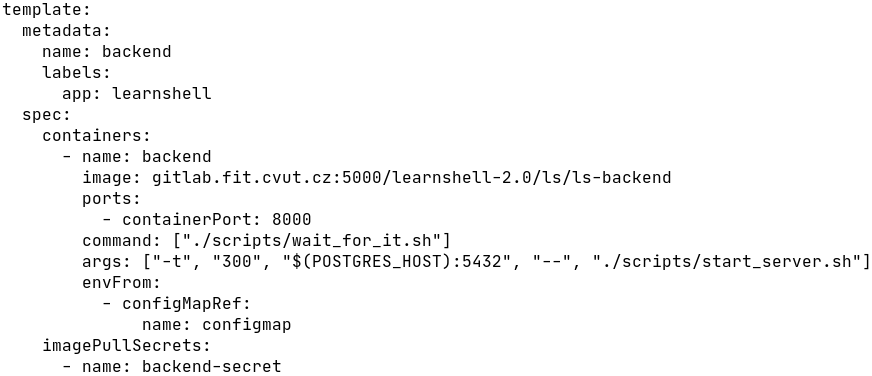
\includegraphics[scale=0.5]{deploy-backend2}
\end{figure}

In this snippet, which is a continuation of the spec field, we have written a \textbf{template} from which our Pods should be built. The template automatically understands that it should build Pods, as it is defined within a Deployment configuration, and inherits its API version as well. Therefore, there is no need to specify either the apiVersion or the kind fields. Within the metadata field, we simply assign the Pod to our learnshell application and give it the same name as the Deployment which manages it.

As for the spec field, there are two key-value pairs: 

\begin{itemize}
  \setlength\itemsep{0em}
  \item \textbf{containers} is mapped to a list of one or more container specifications, defining the containers which should be built within the Pod.
  \item \textbf{imagePullSecrets} is in turn mapped to a list of Secrets in our cluster which we shall be using to authenticate to our Gitlab private registry and pull Docker images from it. As the backend Pod only takes a single container, which contains the code for the backend component, we only need to include the secret to the private registry within our backend repository on Gitlab.
\end{itemize}

Furthermore, let us walk through the \textbf{containers} field, which contains a single container:

\begin{itemize}
  \setlength\itemsep{0em}
  \item \textbf{name} is self-explanatory; it assigns a name by which we can identify our container within the Pod.
  \item \textbf{image} tells the Pod from where to pull the container image. Here, it is the URL of our server and its open port, with the path starting at the LearnShell group, continuing with the repository within that group, and finally the name of the image.
  \item \textbf{ports} is a list of ports that the container should be using, much like in a typical Docker container on any other machine.
  \item \textbf{command} and \textbf{args} is simply a command and a sequence of its arguments that should be run on container start-up. In our case, we first execute a script that runs for 300 seconds until it connects to our PostgreSQL database which is running on another Pod, and on completion, starts serving our Django application.
  \item \textbf{envFrom} is tied to our ConfigMap resources. By using \textbf{configMapRef}, we tell our container to use all the variables contained within the specified ConfigMap. However, it is also possible to handpick the variables to pull from our ConfigMap, if need be.
\end{itemize}

As for our other Deployments, their YAML configurations all follow a very similar pattern to the one we just demonstrated. Each Deployment has its own unique name and its own unique template by which Pods are created, with different ports, start-up scripts, and of course, Docker images. For a closer inspection into our configuration files, see the Gitlab repository for our cluster.

\clearpage

\section{StatefulSets}

Since LearnShell is a stateful application with two different databases (a PostgreSQL database and a Redis key-value cache store), we need a way of ensuring persistent storage in our cluster. This can be done by using StatefulSets in tandem with PersistentVolumeClaims. Better yet, one may notice that there aren't any specific demands we may ask of our databases; besides details such as setting the desired capacity of our PostgreSQL database, our databases should behave exactly like those in any other applications. As such, Helm charts are a very solid choice for our use case, as there is nothing particularly unique in what we want our databases to do, besides the obvious, which is persistent storage of data.

We installed both our PostgreSQL and Redis Helm charts from the Bitnami Helm chart repository, which is maintained (among other Bitnami offerings) by VMWare since the acquisition of Bitnami in 2019. \cite{bitnami} In addition, we have used the Gitlab Helm chart repository for our Gitlab Runners; however, we have dedicated a separate section to our CI/CD process, where they will be expanded upon.

\clearpage

\subsection{PostgreSQL}

\begin{figure}[htbp!]
\centering
\caption{PostgreSQL Helm chart}
\hspace*{0.4cm}
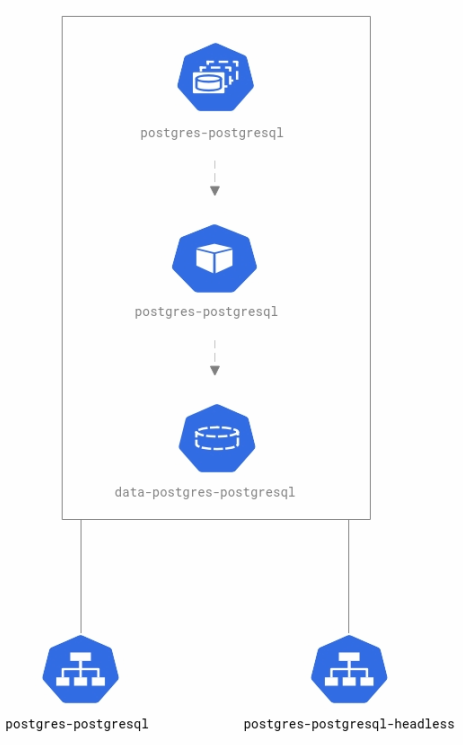
\includegraphics[scale=0.6]{postgres-diagram}
\end{figure}

The above diagram shows the workloads and services generated by our Helm chart, and serves as a perfect example of a basic stateful application in a Kubernetes cluster. After the installation of the PostgreSQL chart, several resources are created; most importantly, a StatefulSet which directly creates and maintains replica Pods, and a PersistentVolumeClaim resource which dynamically allocates storage that persists even after our Pods are deleted.

There are two Services in use here; a "classic" Service which enables the communication between our PostgreSQL Pod and other pods (as seen in the previous section, the backend Pod establishes network communication with the postgres Pod immediately upon the start-up of its container) and a "headless" Service. A headless Service differs from a ClusterIP service (which we are using in our Deployments as well) in that it assigns an IP address to each of our pods, while a ClusterIP service assigns the same IP address to all Pods belonging to a single Deployment (or StatefulSet). \cite{kube-action} In communication between Pods and outside of our cluster, the ClusterIP service is utilized, while during the process of writing to our PostgreSQL database, we use the headless Service. This is because our StatefulSet has to watch out for potential overwrites of the data in our database, and as such it has to process each new write request individually for each Pod; as such, each Pod needs to be identified by its own IP address. In our Values file for this Helm chart, we specified the name of our database as well as the necessary credentials (although more precaution, ideally using a Secret would be preferable in a production cluster). Also, the size of our PersistentVolume (into which the PersistentVolumeClaim writes data) was defined as 20GiB.

\subsection{Redis}

\begin{figure}[H]
\centering
\caption{Redis Helm chart}
\hspace*{-2.2cm}
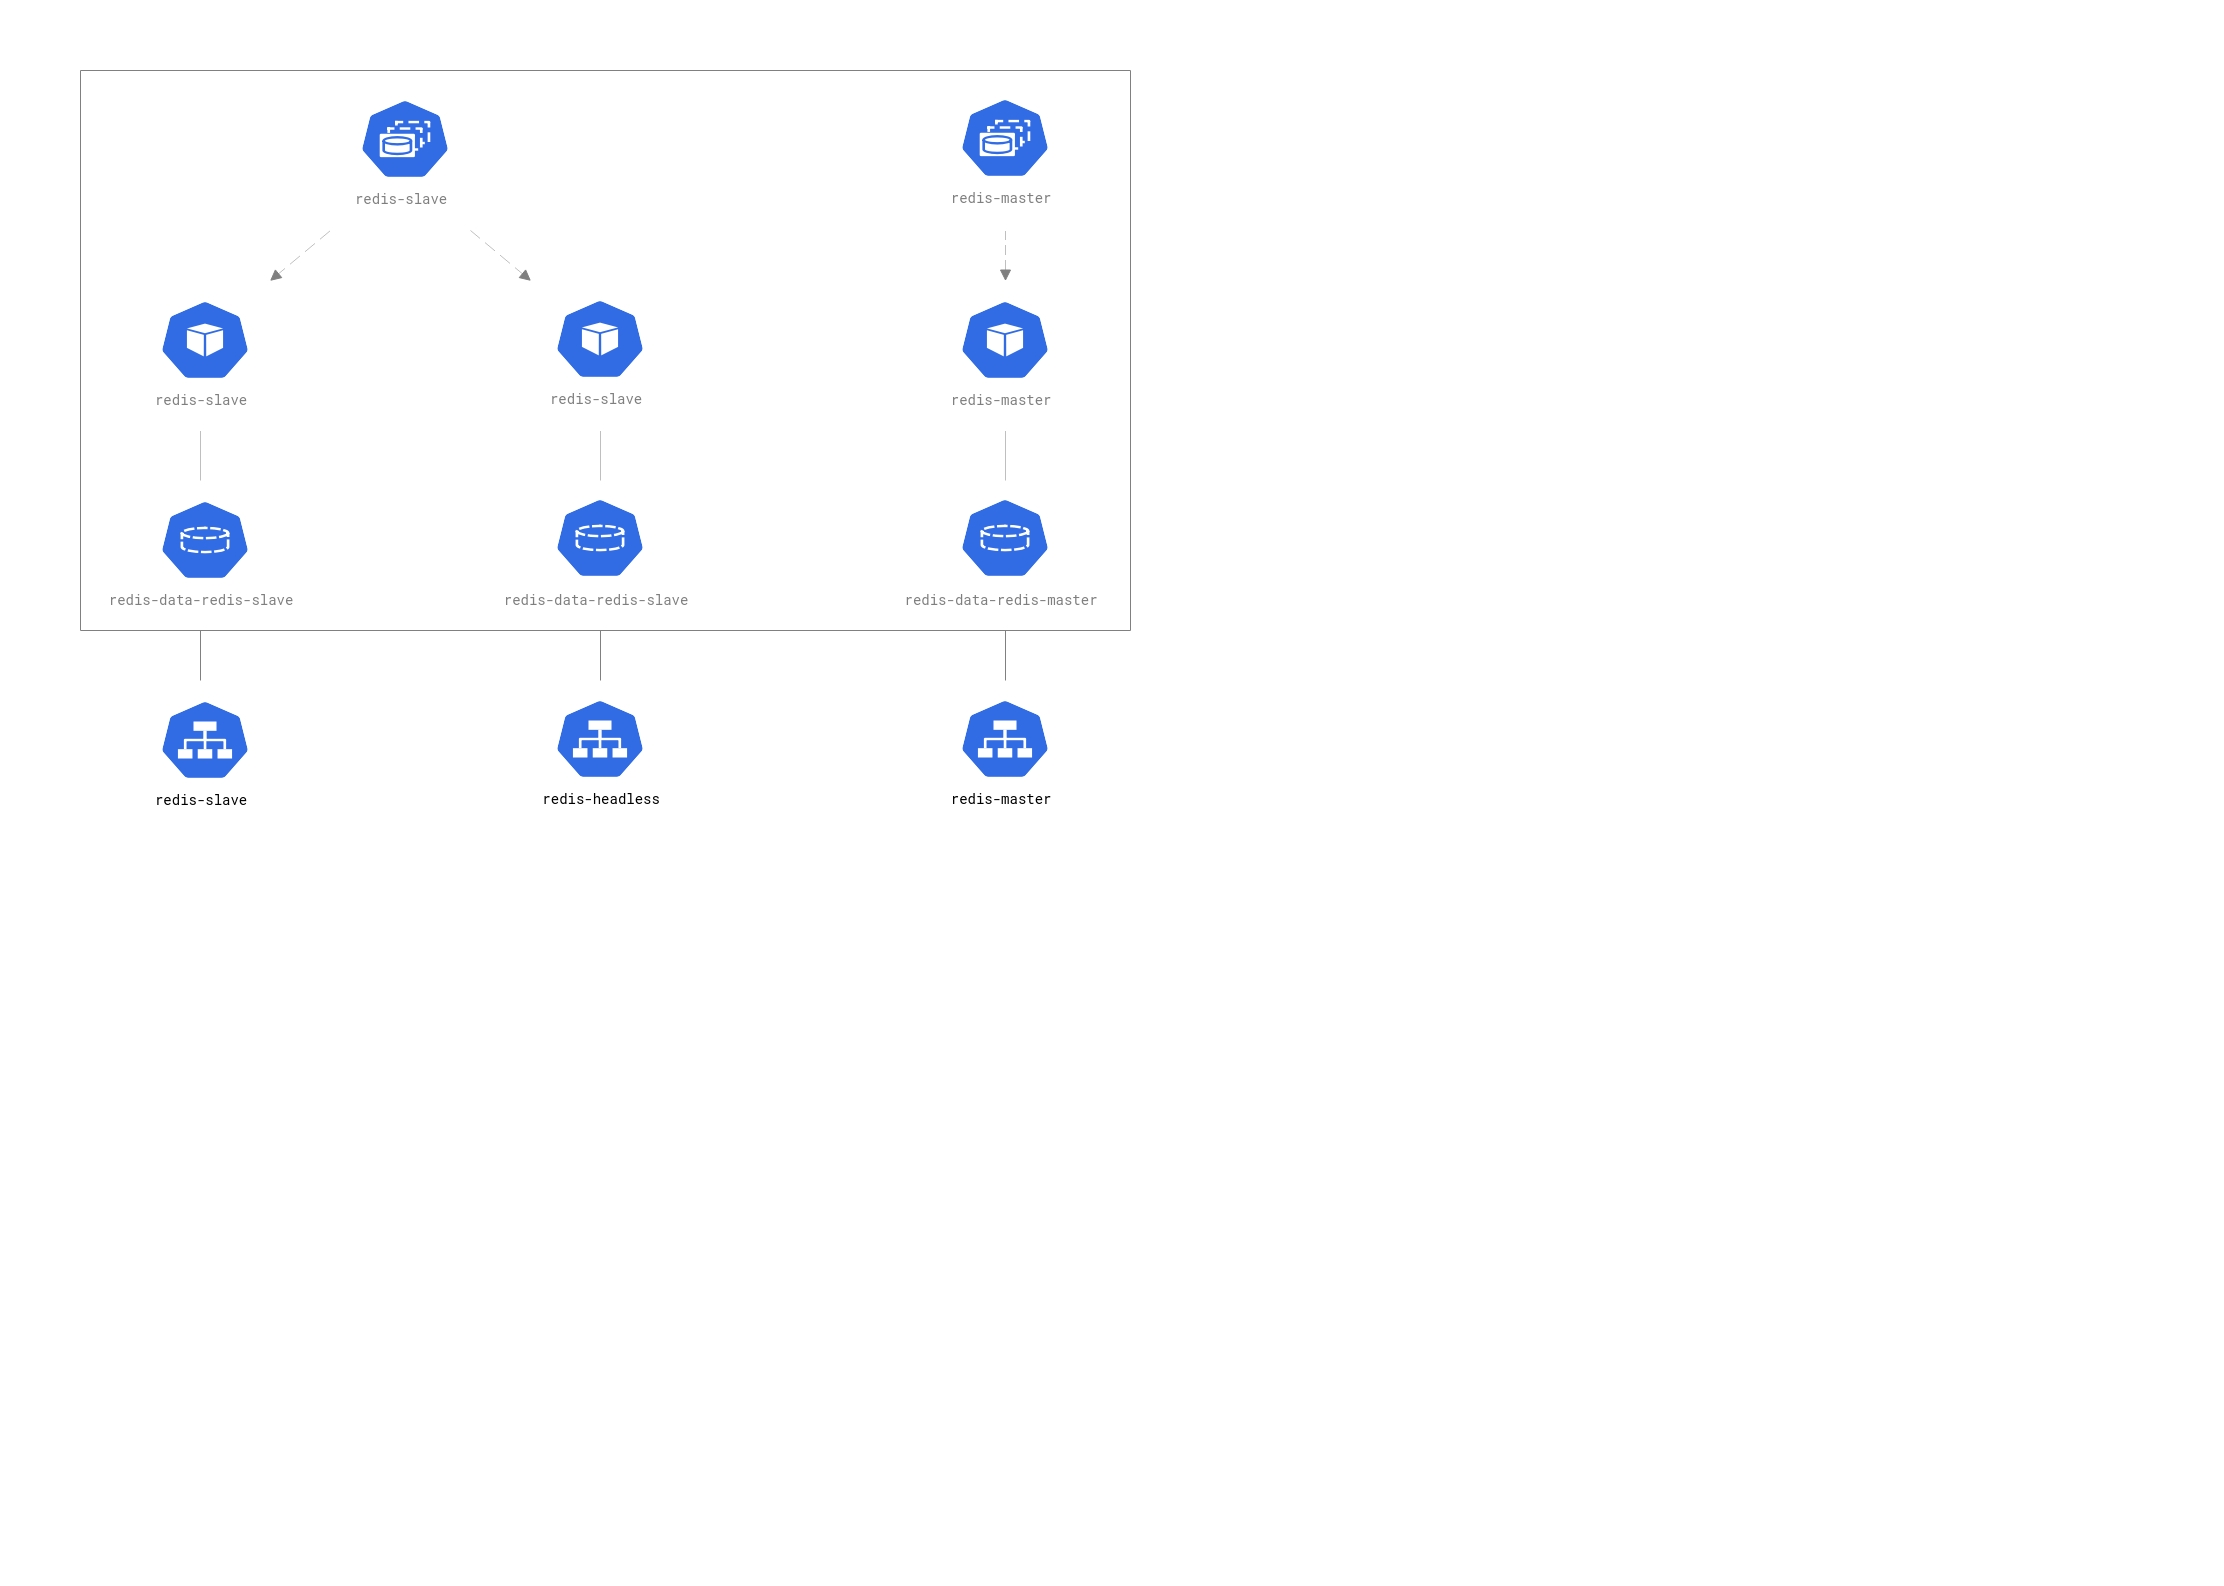
\includegraphics[scale=0.5]{redis-diagram}
\end{figure}

Our second Helm chart represents our Redis cache database. Here, we can see another sizable advantage of using Helm charts, as they can be used to quickly get slightly more complex systems up and running according to best practices; in our case, Bitnami packaged a Redis system with a simple master-slave architecture, containing one Master and two Slave Pods. This is thanks to one of the great features of Kubernetes; since it was built with the goal of assuring high availability and redundancy, it is tailor-made for systems adhering to a master-slave architecture.

In practice, a Redis Master server bears the responsibility of writing new data to Redis Slaves; by continuously synchronizing data with the Redis Master, which serves as a source of truth for our system, redundancy is assured; if one Redis Slave were to cease functioning, another would take its place with no loss of data. On the other hand, for read operations, any Redis Slaves can be used, as these operations cause no changes of data in our database. \cite{redis}

Similarly to our PostgreSQL chart, a headless Service is used to differentiate between Pods when writing to our PersistentVolume. Importantly, there is also one service for our Redis Master and one service for our Redis Slave to allow for seamless communication between them.

\section{Networking}

To enable communication between our Pods over the local cluster network as well as to expose our cluster to the internet, some networking configuration is necessary. In this section, we shall provide an overview regarding the Kubernetes resources (and their configuration) we used to achieve these goals.

\subsection{Services}

As was discussed in the previous chapters, a Kubernetes cluster uses Services to expose applications running on Pods to the network. There are different types of Services, each of them suited for different purposes. In summary, we make use of the following types of services in our cluster:

\begin{itemize}
  \setlength\itemsep{0em}
  \item \textbf{ClusterIP} is the most used by far and serves the purpose of assigning IP addresses to Pods as well as a single DNS name for a set of Pods (such as backend.learnshell.svc.cluster.local), therefore enabling our Deployments to send data to and from each other.
  \item \textbf{NodePort} is almost the same as the ClusterIP Service, except that it also exposes our service to the internet. This Service can be accessed by specifying the IP address of the NodePort and the open port.
  \item \textbf{LoadBalancer} also exposes the service to the internet, with the added bonus of using load balancing to control the incoming traffic more efficiently. To achieve this, it either uses the cloud provider's load balancer or a load balancer which is set up on our on-premises machine.
\end{itemize}

Lastly, we use the Ingress resource to expose our cluster to the internet by providing a specific IP address and DNS name to access our application as a user. 

\subsection{Ingress}

\begin{figure}[H]
\centering
\caption{Ingress Helm chart}
\hspace*{-1cm}
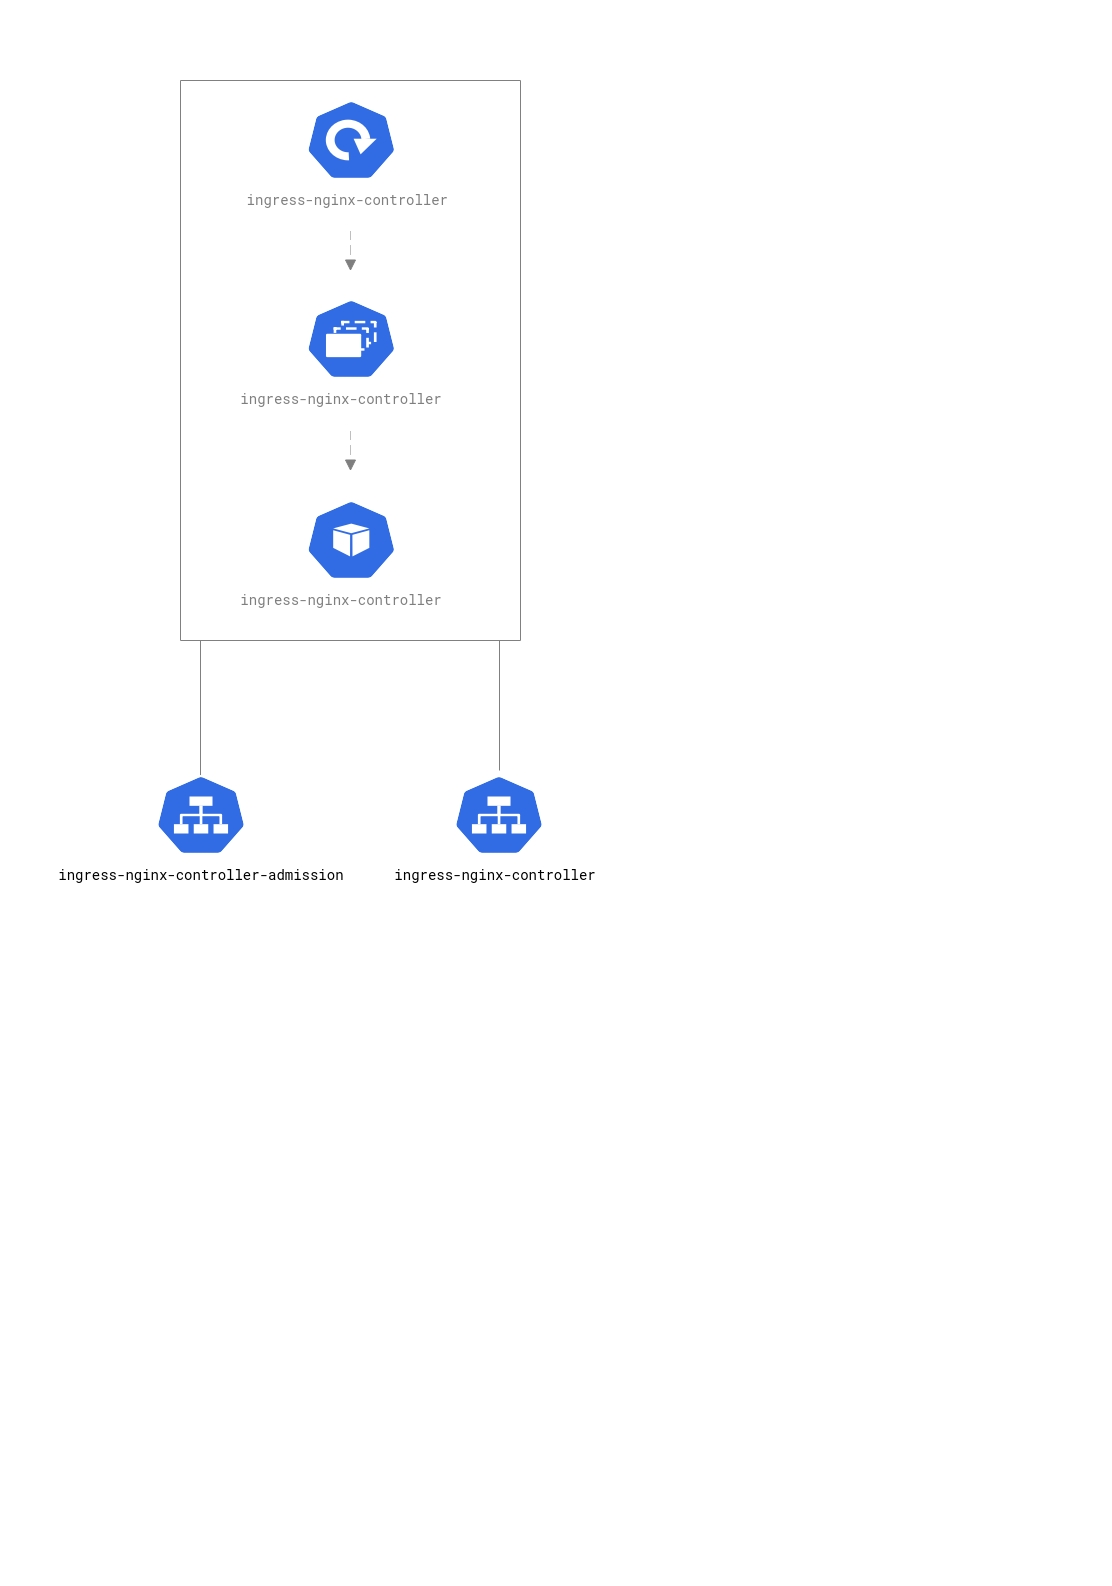
\includegraphics[scale=0.6]{ingress-diagram}
\end{figure}

Much like in the case of our StatefulSets, we have used a Helm chart to set up Ingress for our cluster. As we can see from the diagram, our configuration looks quite similar to a typical Deployment in our cluster, with an important difference in that it also uses a Service dedicated to load balancing of incoming requests.

One of the most important parts of an Ingress configuration is the Ingress controller, which can be in simple terms imagined as a Deployment that facilitates the creation of Pods with specific web server technologies. In fact, there are numerous different controllers maintained as of today, with three controllers (AWS, GCP, and nginx) having official support from the Kubernetes community and many more being maintained by large companies and used in projects all across the world. In this cluster, the nginx controller is used for two reasons; it is completely provider-independent and by far the most convenient to set up due to the current version of LearnShell using an nginx proxy server to forward requests to its components.

\subsection{Ingress configuration}

In addition to the Ingress controller, a working Ingress configuration also requires a resource that serves as a set of rules based on which requests from outside of the cluster are forwarded to specific components of the LearnShell system. These rules are outlined in a configuration file which we shall analyze in this subsection. As in the Deployment section, let us take a closer look at this file.

\begin{figure}[H]
\centering
\hspace*{0.7cm}
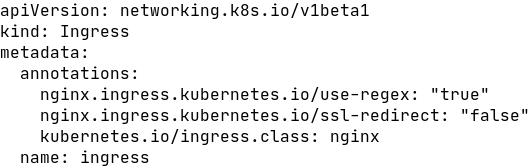
\includegraphics[scale=0.5]{kube-ingress1}
\end{figure}

As in our Deployments, there are four required fields, which fulfill the same function as in any other resource:

\begin{itemize}
  \setlength\itemsep{0em}
  \item \textbf{apiVersion} here is different from the others in our cluster; instead of v1, v1beta1 is used. The reason is that in order to make our Ingress configuration work on both GCP and on-premises, we unfortunately can not use the newest version of the Kubernetes API, as it is not supported yet by GCP. Therefore, we have to use v1beta1, an older version of the API which is quite different from v1 in regards to the syntax of configuration files. Nevertheless, as soon as cloud providers start using v1 for Ingress, there is no reason not to migrate to that version in our cluster as well.  
  \item \textbf{kind} is much the same as anywhere else, simply denoting the kind of resource we want to create.
  \item \textbf{annotations} provides our Ingress with additional information in regards to functionality. Here, we specified that regular expressions should be used in the rules inside our spec value, that no SSL redirection should be used at the moment as the current version of our cluster does not use HTTPS (of course, this can and will be configured once the cluster is used in production) and that we are using the nginx controller, here told inside the ingress.class key-value pair.
  \item \textbf{name} is self-explanatory.
\end{itemize}

\begin{figure}[H]
\centering
\hspace*{0.7cm}
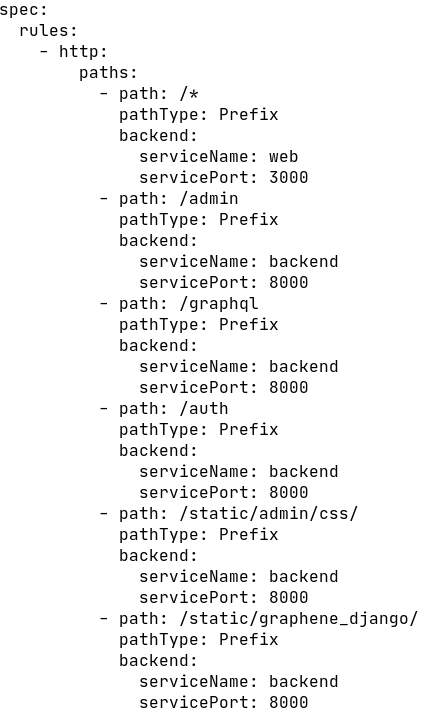
\includegraphics[scale=0.5]{kube-ingress2}
\end{figure}

The spec field is, as usual, the longest part of our configuration file. In an Ingress resource, it mandatorily contains the rules by which our network should abide when handling requests from outside. However, there are many other options to configure, such as the DNS name that should be translated into the IP address which serves as the root of our application website. In our case, there is no host, but should the cluster be used in practice, it would be set to the current website of the LearnShell portal.

In any case, we command Ingress to route any requests received via the HTTP protocol based on the specified path. The first path, which translates to \verb|http://<ip addr>/*| uses the asterisk wildcard to redirect any request to the web Pod using port 3000 (on which our JavaScript front end is exposed). In the paths below, special cases, are specified, such as \verb|/admin|. In case the request is made to that path, it is redirected directly to our back end instead. These rules are also used for static files; if the client requests a CSS file within the \verb|/static/admin/css| path, for example, it is retrieved from that very folder inside the container running inside of our backend Pod.


\section{Private container registry}

As we have decided to use the Gitlab Container Registry to store our Docker images, this process will be dedicated to showing our process of setting it up. 
Since container registries are not enabled by default on Gitlab, we need to enable it in the permissions of each repository which should have its own registry. In addition, we need to generate a deploy token with read registry access for each Gitlab repository. We shall use it later to authenticate from our cluster. Both of these tasks can be completed by using the web GUI of the Gitlab server. After these fairly straightforward tasks, we should reiterate why we require a registry for our cluster.

\subsection{Authentication}

Firstly, we want the Pods in our cluster to \textbf{pull} images from our registry, which shall be used as templates for the containers running within them. Secondly, in order to keep our cluster up-to-date, we want to \textbf{push} newly built images into our registry for the cluster to pull from. 

To pull as well as push from a private container registry as a developer, one merely needs to authenticate using \verb|docker login <registry url>| and providing his credentials to prove he has the necessary privileges. However, to make a Pod inside our cluster pull images from that same registry automatically as part of its lifecycle, some additional configuration is needed. According to the Kubernetes documentation, a Pod should use a Secret to authenticate to private registries. Thus, we have created Secrets for each repository which is part of the LearnShell group, so that the generator Deployment can pull a Docker image from the Gitlab repository containing the code for the generator, and likewise for our other Deployments.

The Secret should contain a key-value pair, binding the key named ".dockerconfigjson" to a value that represents a base64 encoded Docker configuration file containing only the authentication data for our registry. See the image below for an example of such a file, which we wrote purely for didactic purposes.

\begin{figure}[H]
\centering
\hspace*{-0.6cm}
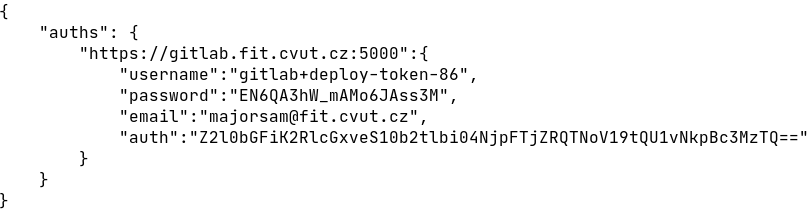
\includegraphics[scale=0.5]{docker-config}
\end{figure}

As we can see from this figure, the file is in JSON format. The first key-value pair, with the key "auths" refers to a collection (in JSON nomenclature, the exact term is object) of more key-value pairs, in this case only consisting of one pair. This pair uses the URL of the registry as well as the port on which Gitlab exposes it. As the associated value, there is an object consisting of the following:

\begin{itemize}
  \setlength\itemsep{0em}
  \item \textbf{username}, in this case, represented by the name of our deploy token with read registry access
  \item \textbf{password} as the value of the deploy token
  \item \textbf{email} can be any email with at least developer access in the group to which the registry belongs (in this case LearnShell 2.0 on Gitlab)
  \item \textbf{auth} is merely the output of \verb|base64 <<< <username>:<password>|
\end{itemize}

Finally, by base64 encoding the Docker configuration file, we receive the desired value of .dockerconfigjson in our Secret. By following these guidelines, we have created Secrets for all of our registries, and our Pods can hereby pull images from them.

Since our CI/CD process necessitates the pushing of images into our registries, it is imperative that they can be accessed from our pipelines. Thankfully, this is a much less time-consuming task, as Gitlab CI provides us with built-in variables CI\_REGISTRY\_USER, CI\_REGISTRY\_PASSWORD, and CI\_REGISTRY, which provide us with the username to push containers to the registry, a password which is newly generated (and valid) for each job and the URL, as well as port, if one is specified in the registry configuration.

\subsection{Potential improvements}

As of right now, we are using multiple registries, one per every repository in the LearnShell 2.0 group on Gitlab. Using one group registry for all of our repositories would be much easier to manage since we wouldn't need to have multiple Secrets on our cluster for each registry. Unfortunately, this is not possible in the current version of Gitlab used by the Czech Technical University, which is Gitlab 11.8.10. Additionally, if we tried to circumvent this problem by simply specifying a dummy repository with the sole purpose of hosting our registry, we would encounter issues with authentication; the built-in variables defined in the previous section can be only applied to a registry hosted in the repository in which the CI/CD pipeline is defined. Therefore, we have no choice but to run multiple registries. Nevertheless, this is not a problem functionality-wise; it is merely a quality of life issue regarding the number of Secrets which we have to maintain.

However, group level registries were introduced in Gitlab 12.10, and are specifically designed to provide a single registry for the entire group, with each repository being able to access the registry in its CI/CD pipeline. Once our university upgrades its Gitlab version, it would be trivial to move from project level to group level registries.


\section{CI/CD implementation}

Finally, it is time to direct our attention to the implementation of a CI/CD pipeline by making use of several of the tools from the large toolbox which is the Gitlab CI offering. As we have described our goals, as well as the general structure of our pipelines in the previous chapter, we will directly jump into the implementation. We have implemented CI/CD routines for the front end, back end, celery, and generator Deployments.

To create a functioning CI/CD pipeline, there are two preliminary steps: writing a configuration file from which a pipeline will be constructed and provisioning an environment on which to run jobs that are contained within the pipeline.

\subsection{Gitlab Runners}

According to the Gitlab documentation, a Gitlab Runner is an application that works with Gitlab CI to run jobs inside pipelines. This application can be deployed to several different operating systems, and it is entirely up to decide whether to install it as a package, container, or as a Helm chart.

By installing it as Helm chart in our cluster, we not only make our work a bit easier for ourselves, as we avoid having to provision a VM for our runners, but we also make use of an extremely useful boon; as the runners would now belong to our cluster, we can configure them to have specific privileges, such as updating Deployments or deleting Pods. The Helm chart for a Gitlab Runner can be installed much like any other chart; one adds a chart repository (here provided by Gitlab) and installs it from the repository, optionally supplying it with a Values file. Provided below is an example of such a file.

\begin{figure}[H]
\centering
\hspace*{-0.6cm}
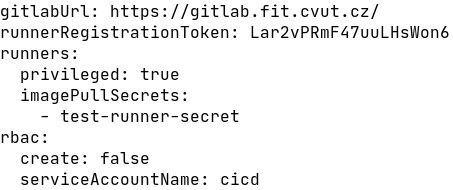
\includegraphics[scale=0.5]{runner-values}
\end{figure}

The gitlabUrl value is tied to the URL of the server on which Gitlab is running, while the runnerRegistrationToken is a unique token that maps the Helm chart to the repository in which we want to run our pipeline. Under runners, setting the privileged value to true allows our runner to run docker commands, such as \verb|docker exec|, which we will be using for running unit tests, and imagePullSecrets is much the same as in our other Pods, in that it assigns a Secret to the Pod on which the runner is deployed which authenticates it to pull Docker containers from a private registry during our CI/CD jobs.

The values under rbac (this acronym stands for role-based access control) are a bit more complicated; create is mapped to a boolean which essentially tells the Helm chart if we want to create a special ServiceAccount for the Pod on which the chart is running. The value of serviceAccountName in turn specifies which ServiceAccount to associate with the Pod; if we don't include a value, the default ServiceAccount of the cluster is used. On another note, if we allow the chart to create a ServiceAccount by itself (we can assign privileges to it via the same Values file), this would mean that each runner in its cluster would have its very own ServiceAccount. While this is not a problem from a functionality-based viewpoint and neither is it a security concern, we save our future selves some work by configuring a ServiceAccount on our own, as this would mean that if we wanted to change up some privileges for our runners, we only have to edit a single file (that which configures the privileges for our account). Using the default ServiceAccount would be a bad practice, as that account is used by all our other Pods; even though we want to give our Pods with Gitlab Runners the privilege of manipulating Deployments, that doesn't mean we would like to allow any other pods to tamper with these Deployments as well. Therefore, we have created a special ServiceAccount called "cicd", which is bound to an equally named Role via a RoleBinding. This Role only allows cicd to perform updates on Deployments, and nothing else. 



\subsection{CI/CD pipeline configuration}

The second step in setting up our CI/CD process is actually defining our pipeline. We will use the pipeline for our front end Deployment as a demonstration of our CI/CD implementation, as it already contains a collection of unit tests we can execute as part of our CI process. As we have discussed beforehand, in Gitlab CI, CI/CD pipelines are divided into jobs, which are defined in a configuration file in the root of the project, by default named. gitlab-ci.yml. Let us walk through the .gitlab-ci.yml file for the LS Web repository, which contains the JavaScript code for the LearnShell front end.

\begin{figure}[H]
\centering
\hspace*{-0.6cm}
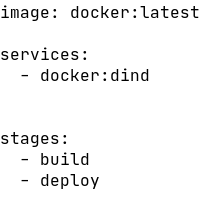
\includegraphics[scale=0.5]{gitlab-ci-stages}
\end{figure}

At the start of our file, by setting the image to docker:latest, we demand that the runner creates a Docker container in which to run the now isolated pipeline. Additionally, by specifying docker:dind as a service, Docker-in-Docker is installed into our container, which enables our container to build Docker images. The "stages" keyword defines a sequence of stages (essentially groups of jobs), with a caveat that if the current stage doesn't succeed, our pipeline does not move on to the next one. Let us continue with the definition of the "build" job.

\begin{figure}[H]
\centering
\hspace*{-0.3cm}
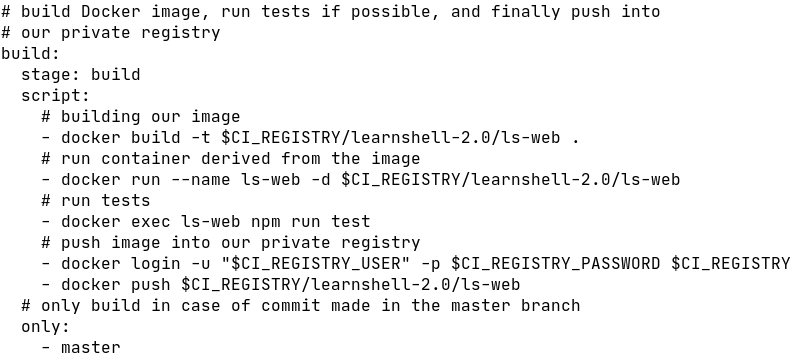
\includegraphics[scale=0.5]{gitlab-ci-build}
\end{figure}

As we can see from the code, this job is dedicated to the build stage of our pipeline. Following the analysis from our previous chapter, this job does most of the grunt work of our pipeline. It builds our Docker image, runs a container, immediately executes unit tests on it, and finally pushes the newly built image into our private registry. The last part, that is the "only" keyword, serves to notify our runner to only run this job if the commit is pushed into the master branch of our repository.

\begin{figure}[H]
\centering
\hspace*{-0.5cm}
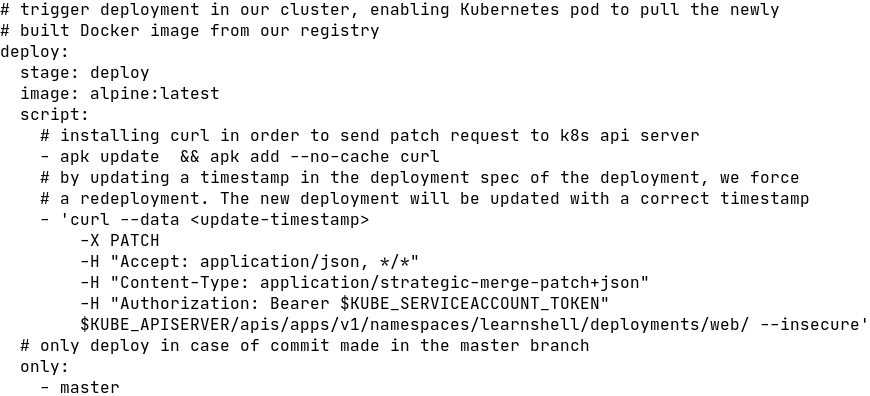
\includegraphics[scale=0.5]{gitlab-ci-deploy}
\end{figure}

The last stage in our pipeline is the deploy stage, as defined here. Here, we pull the image of Alpine Linux, which is a minimalistic Linux distribution used extremely commonly as a sort of empty container without any additional pre-installed programs beyond what is absolutely necessary. In the container that is created for us, we install the shell utility "curl", which is a commonly used tool to transfer data to and from servers. By using curl, we send a PATCH request to the IP address of the API server of our cluster. This request contains data that would update the timestamp of our Deployment (marked as <update-timestamp> because it is needlessly long for this demonstration), and authenticate using a ServiceAccount token, which we retrieved manually from our pod and saved into a Gitlab project variable. This solution might be rather obfuscated; another option is to install kubectl and use it to restart the Deployment. However, that solution would be slower for the runner to execute, since it installs additional software that is not really necessary for a simple request to the cluster API.

As for the other repositories, their pipelines are almost completely identical to this one, with their .gitlab-ci.yml files only differing in minutiae regarding names of images and Deployments. 

\subsection{Potential improvements}

While we are quite satisfied with our current CI/CD process, we are still slightly constrained by the version of Gitlab in use by the university. There are two features we could make use of in the future if newer versions are used; group variables and running of jobs after a commit is merged into a branch. Currently, the environmental variables KUBE\_SERVICEACCOUNT\_TOKEN and KUBE\_APISERVER are the same across all repositories, since we are using the same ServiceAccount for all our runners. Therefore, it would be preferable to have a single place from which to set this variable globally for the group. Unfortunately, this is only available in the later versions of Gitlab. Furthermore, our current pipelines are devised so that their jobs only run when a commit is made into the master branch. Ideally, we would like these jobs to run only after a merge request is accepted into that branch. As with group variables, the issue lies in the fact that running jobs post-merge is not available in our version. Still, pushes into master are almost always made in the form of merges from other branches, and as such, this isn't at all a pressing issue.

As in the previous section, these improvements are merely quality of life ones; our goals are fully achieved with the tools on offer by our version of Gitlab.

\setsecnumdepth{part}
\chapter{Conclusion}

In closing, let us walk through the goals set in this thesis. 

In the first chapter, we reviewed the current infrastructure architecture of LearnShell, and proposed possible improvements. Then, we have gone over the theoretical concepts behind modern cluster platforms and talked about some of the most used technologies in the field. Afterwards, we analyzed and scrutinized the suitability of technologies that would help us create that cluster, and used our acquired knowledge to create a project that would create a cluster from a combination of configuration files and commands, allowing the user to choose between an on-premises cluster and a cloud-based one (while discussing the pros and cons of each). Finally, as our last task, we implemented a CI/CD pipeline for each project where it was deemed necessary, by using our newly created cluster to deploy Gitlab Runners. Additionally, we provided diagrams as well as code snippets from our project in order to shed light on our cluster infrastructure as well as our CI/CD process. 

In order to achieve our aims, we have used many different technologies, though there was a special focus on Docker, Kubernetes, and Gitlab CI for containerization, orchestration, and CI/CD respectively.

The code is available for students and staff on a repository in the Gitlab server of the Czech Technical University in Prague. Moreover, we have organized the Docker images into private registries on Gitlab and built pipelines around them via Gitlab CI.

While we feel confident that the goals were completed, there is always room for improvement; in this current iteration, the cluster can be used in practice as a staging environment for development, but to be truly production-ready, some additional work would be required, mainly in regards to networking. Nonetheless, we believe that in this state, LearnShell is well-situated to migrate completely to a cluster infrastructure in the near future.



\bibliographystyle{iso690}
\bibliography{citations}


\setsecnumdepth{all}
\appendix

\chapter{Acronyms}
% \printglossaries
\begin{description}
	\item{API} Application Programming Interface
	\item{CD} Continuous Delivery
	\item{CI} Continuous Integration
	\item{CSS} Cascading Style Sheets
	\item{GCP} Google Cloud Platform
	\item{GKE} Google Kubernetes Engine
	\item{GUI} General User Interface
	\item{HTTP} Hypertext Transfer Protocol
	\item{HTTPS} Hypertext Transfer Protocol Secure
	\item{IP} Internet Protocol
	\item{JSON} JavaScript Object Notation
	\item{K8S} Kubernetes
	\item{URL} Uniform Resource Locator
	\item{VM} Virtual Machine
	\item{YAML} YAML Ain't Markup Language
	
\end{description}

\chapter{Kubernetes diagram legend}
% \printglossaries
\begin{figure}[H]
\centering
\hspace*{-0.5cm}
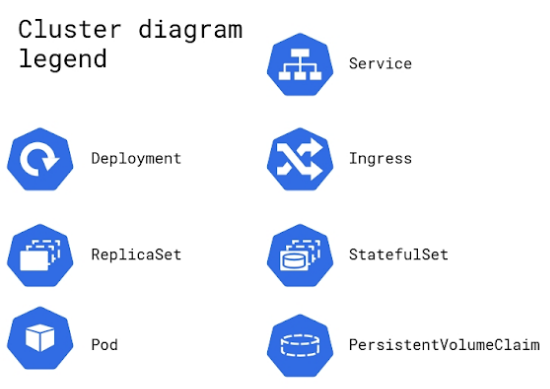
\includegraphics[scale=0.7]{legend}
\end{figure}


\chapter{Contents of enclosed CD}

%change appropriately

\begin{figure}
	\dirtree{%
		.1 readme.txt\DTcomment{description of the contents of the CD}.
		.1 ls-cluster\DTcomment{repository containing the cluster configuration}.
		.1 cicd\DTcomment{directory containing gitlab-ci.yml files used for CI/CD}.
		.1 assignment.pdf\DTcomment{assignment in PDF format}.
		.1 thesis.pdf\DTcomment{thesis in PDF format}.
	}
\end{figure}

\end{document}
